% ======================================================================
%  Soutenance de stage -- Master 2 SAR -- Dan CALAMIA -- Septembre 2026
%  Cartographie sémantique coopérative multi-robots par fusion LiDAR-caméra
% ----------------------------------------------------------------------
%  Compilation : pdfLaTeX, deux passes (ou : latexmk -pdf main.tex)
%  Images      : dossier Images/ du rapport, à placer à côté de main.tex
%                (mêmes noms de fichiers que dans le rapport).
%  Oral        : les blocs "% À DIRE" avant chaque slide résument ce qu'il
%                faut dire ; la durée indiquée est approximative
%                (total visé : ~20 min, hors questions).
%  Format 4:3  : remplacer aspectratio=169 par aspectratio=43
%                (les schémas sont pensés pour le 16:9).
% ----------------------------------------------------------------------
%  Fichiers :
%    style.tex            thème (couleurs, polices, gabarits)
%    01_contexte.tex      contexte, problématique, objectifs
%    02_liosam.tex        SLAM, LIO-SAM (principe, architecture, choix)
%    03_yolo.tex          YOLO (principe, segmentation sémantique)
%    04_framework.tex     framework de fusion LiDAR-caméra
%    05_extensions.tex    loop closure, carte a priori, multi-robots
%    06_resultats.tex     expérimentations et résultats
%    07_conclusion.tex    bilan, perspectives, questions
%    08_annexes.tex       slides de secours pour les questions
% ======================================================================
\documentclass[aspectratio=169,11pt]{beamer}
% ======================================================================
%  style.tex -- Thème de la présentation (couleurs, polices, gabarits)
%  Chargé par main.tex avec % ======================================================================
%  style.tex -- Thème de la présentation (couleurs, polices, gabarits)
%  Chargé par main.tex avec % ======================================================================
%  style.tex -- Thème de la présentation (couleurs, polices, gabarits)
%  Chargé par main.tex avec \input{style}.
%  Couleur principale : primaryblue, la même que dans le rapport.
% ======================================================================

% ---------------------------------------------------------------------
%  Encodage et langue
% ---------------------------------------------------------------------
\usepackage[utf8]{inputenc}
\usepackage[T1]{fontenc}
\usepackage[french]{babel}

% ---------------------------------------------------------------------
%  Polices : Fira Sans si elle est installée (Overleaf, TeX Live complet),
%  sinon Latin Modern. Les formules restent en police à empattements.
% ---------------------------------------------------------------------
\IfFileExists{FiraSans.sty}{\usepackage[sfdefault]{FiraSans}}{\usepackage{lmodern}}
\usefonttheme[onlymath]{serif}

% ---------------------------------------------------------------------
%  Paquets
% ---------------------------------------------------------------------
\usepackage{graphicx}
\usepackage{adjustbox}   % \adjincludegraphics : recadrage des images en % de leur taille
\usepackage{amsmath,amssymb}
\usepackage{booktabs}
\usepackage{pifont}      % symboles coche / croix
\usepackage{tcolorbox}
\tcbuselibrary{skins,raster}
\usepackage{tikz}
\usetikzlibrary{positioning,arrows.meta,shapes.geometric,calc,fit,backgrounds,babel}

% Images : même dossier "Images" que le rapport (à côté de main.tex,
% ou un niveau au-dessus si la présentation est un sous-dossier du rapport)
\graphicspath{{Images/}{../Images/}}

% ---------------------------------------------------------------------
%  Couleurs
% ---------------------------------------------------------------------
\definecolor{primaryblue}{RGB}{20,60,110}   % bleu du rapport
\definecolor{accent}{RGB}{230,115,25}       % orange de mise en valeur
\definecolor{softblue}{RGB}{233,239,247}    % fond clair
\definecolor{textgray}{RGB}{100,100,100}    % gris du rapport
\definecolor{okgreen}{RGB}{40,140,80}
\definecolor{kored}{RGB}{200,45,45}
% Classes sémantiques (mêmes codes couleur que les cartes du rapport)
\definecolor{cRoute}{RGB}{40,40,40}
\definecolor{cBati}{RGB}{215,50,50}
\definecolor{cVege}{RGB}{50,150,60}
\definecolor{cAutre}{RGB}{150,150,150}
\definecolor{cVoiture}{RGB}{105,70,200}
\definecolor{cCiel}{RGB}{110,170,230}
% Facteurs de LIO-SAM (mêmes couleurs que la figure liosam2.png)
\definecolor{fIMU}{RGB}{238,134,48}
\definecolor{fLidar}{RGB}{120,176,72}
\definecolor{fGPS}{RGB}{214,190,40}
\definecolor{fLoop}{RGB}{25,25,25}

% ---------------------------------------------------------------------
%  Réglages généraux Beamer
% ---------------------------------------------------------------------
\setbeamertemplate{navigation symbols}{}
\hyphenpenalty=10000 \exhyphenpenalty=10000   % pas de césure sur les slides
\setbeamersize{text margin left=0.9cm, text margin right=0.9cm}

\setbeamercolor{normal text}{fg=black!85, bg=white}
\setbeamercolor{structure}{fg=primaryblue}
\setbeamercolor{alerted text}{fg=accent}
\setbeamercolor{frametitle}{fg=white, bg=primaryblue}
\setbeamercolor{title}{fg=primaryblue}
\setbeamercolor{subtitle}{fg=textgray}
\setbeamercolor{footline}{fg=textgray}
\setbeamercolor{itemize item}{fg=accent}
\setbeamercolor{itemize subitem}{fg=textgray}
\setbeamercolor{enumerate item}{fg=accent}
\setbeamercolor{block title}{fg=white, bg=primaryblue}
\setbeamercolor{block body}{fg=black!85, bg=softblue}

\setbeamerfont{frametitle}{size=\large, series=\bfseries}
\setbeamerfont{title}{size=\LARGE, series=\bfseries}
\setbeamerfont{subtitle}{size=\normalsize}
\setbeamerfont{footline}{size=\tiny}
\setbeamerfont{alerted text}{series=\bfseries}
\setbeamerfont{itemize/enumerate subbody}{size=\small}

\setbeamertemplate{itemize item}[square]
\setbeamertemplate{itemize subitem}{\textendash}
\setbeamertemplate{enumerate item}{\textbf{\insertenumlabel.}}
\setbeamertemplate{blocks}[rounded][shadow=false]

% ---------------------------------------------------------------------
%  Barre de titre (pleine largeur) + barre de progression orange
% ---------------------------------------------------------------------
\makeatletter
\newlength{\pb@longueur}
\newcommand{\pb@barre}{%
  \setlength{\pb@longueur}{\paperwidth}%
  \ifnum\c@framenumber<\insertmainframenumber\relax
    \setlength{\pb@longueur}{\dimexpr\paperwidth*\c@framenumber/\insertmainframenumber\relax}%
  \fi
  \hbox{{\color{accent}\rule{\pb@longueur}{1.8pt}}%
        {\color{softblue}\rule{\dimexpr\paperwidth-\pb@longueur\relax}{1.8pt}}}%
}
\setbeamertemplate{frametitle}{%
  \nointerlineskip%
  \begin{beamercolorbox}[wd=\paperwidth, sep=0pt, leftskip=0.9cm, rightskip=0.9cm]{frametitle}%
    \usebeamerfont{frametitle}\rule{0pt}{2.9ex}\insertframetitle\rule[-1.5ex]{0pt}{0pt}%
  \end{beamercolorbox}%
  \nointerlineskip%
  \pb@barre%
}

% ---------------------------------------------------------------------
%  Pied de page : auteur | titre court ............ numéro / total
% ---------------------------------------------------------------------
\setbeamertemplate{footline}{%
  \leavevmode%
  \hbox to \paperwidth{%
    \hspace*{0.9cm}%
    \usebeamerfont{footline}\usebeamercolor[fg]{footline}%
    \insertshortauthor\hspace{0.6em}\textbar\hspace{0.6em}\insertshorttitle%
    \hfill%
    \ifbeamer@inappendix Annexe\else\insertframenumber\,/\,\insertmainframenumber\fi%
    \hspace*{0.9cm}}%
  \vspace*{0.28cm}%
}
\makeatother

% ---------------------------------------------------------------------
%  Page de titre
%  (logos : logo_etablissement.png à gauche, logo_labo.png à droite)
% ---------------------------------------------------------------------
\newcommand{\typedocument}{}   % défini dans main.tex
\setbeamertemplate{title page}{%
  \hbox to \textwidth{%
    \adjincludegraphics[height=1.05cm, trim={{0.04\width} {0.31\height} {0.04\width} {0.31\height}}, clip]{logo_etablissement.png}%
    \hfill
    
\includegraphics[height=1.05cm]{logo_labo.png}}%
  \vspace{0.6cm}
  {\small\color{textgray}\typedocument\par}
  \vspace{0.2cm}
  {\usebeamerfont{title}\usebeamercolor[fg]{title}\inserttitle\par}
  \vspace{0.15cm}
  {\color{accent}\rule{2.6cm}{2pt}\par}
  \vspace{0.15cm}
  {\usebeamerfont{subtitle}\usebeamercolor[fg]{subtitle}\insertsubtitle\par}
  \vspace{0.45cm}
  {\large\bfseries\insertauthor\par}
  \vspace{0.1cm}
  {\footnotesize\color{textgray}\insertinstitute\par}
  \vspace{0.1cm}
  {\footnotesize\color{textgray}\insertdate\par}
}

% ---------------------------------------------------------------------
%  Plan : numéros dans des pastilles orange
% ---------------------------------------------------------------------
\setbeamertemplate{section in toc}{%
  \leavevmode\tikz[baseline=(n.base)]\node[fill=accent, text=white, rounded corners=2pt,
    inner sep=2.5pt, minimum width=1.4em, font=\small\bfseries] (n) {\inserttocsectionnumber};%
  \hspace{0.6em}{\color{primaryblue}\inserttocsection}\par}
\setbeamertemplate{subsection in toc}{}

% ---------------------------------------------------------------------
%  Page d'intercalaire au début de chaque partie
% ---------------------------------------------------------------------
\setbeamertemplate{section page}{%
  \begin{minipage}{0.8\textwidth}
    \raggedright
    {\fontsize{40}{40}\selectfont\bfseries\color{accent}%
      \ifnum\value{section}<10 0\fi\arabic{section}\par}
    \vspace{0.3cm}
    {\LARGE\bfseries\color{primaryblue}\insertsectionhead\par}
    \vspace{0.35cm}
    {\color{accent}\rule{3cm}{2pt}\par}
  \end{minipage}%
}
\AtBeginSection[]{%
  \begin{frame}[plain, noframenumbering]
    \vfill\sectionpage\vfill
  \end{frame}
}

% ---------------------------------------------------------------------
%  Petites commandes utiles
% ---------------------------------------------------------------------
\newcommand{\ok}{\textcolor{okgreen}{\ding{51}}}        % coche verte
\newcommand{\ko}{\textcolor{kored}{\ding{55}}}          % croix rouge
\newcommand{\legende}[1]{{\scriptsize\color{textgray}#1\par}}

% Carte (encadré) réutilisable : \begin{tcolorbox}[carte, title=...]
\tcbset{
  carte/.style={enhanced, colback=softblue, colframe=primaryblue, boxrule=0.6pt, arc=4pt,
    colbacktitle=primaryblue, coltitle=white, fonttitle=\bfseries\small, halign title=center,
    fontupper=\small, halign=center, valign=center, left=4pt, right=4pt, top=5pt, bottom=5pt},
  question/.style={enhanced, colback=white, colframe=accent, boxrule=1pt, arc=4pt,
    fontupper=\normalsize, halign=center, left=6pt, right=6pt, top=4pt, bottom=4pt},
}

% ---------------------------------------------------------------------
%  Styles TikZ communs aux schémas
% ---------------------------------------------------------------------
\tikzset{
  >={Latex[length=2mm]},
  boite/.style={draw=primaryblue, fill=white, rounded corners=3pt, align=center,
    font=\scriptsize, inner sep=3pt, minimum height=0.8cm, text width=#1},
  boite/.default=2cm,
  capteur/.style={draw=primaryblue!60, fill=softblue, align=center,
    font=\scriptsize, inner sep=3pt, minimum height=0.7cm, text width=#1},
  capteur/.default=1.5cm,
  donnee/.style={draw=accent, fill=accent!10, rounded corners=3pt, align=center,
    font=\scriptsize, inner sep=3pt, minimum height=0.8cm, text width=#1},
  donnee/.default=2cm,
  sortie/.style={draw=accent, fill=accent, text=white, rounded corners=3pt, align=center,
    font=\scriptsize\bfseries, inner sep=3pt, minimum height=0.8cm, text width=#1},
  sortie/.default=2cm,
  fleche/.style={->, thick, draw=primaryblue!80},
  groupe/.style={draw=primaryblue!45, dashed, rounded corners=6pt, inner sep=5pt},
}

% Facteur de LIO-SAM : \facteur{couleur}{nom}{description}
\newcommand{\facteur}[3]{%
  \begin{tabular}{@{}c@{}}
    \tikz[baseline=-0.6ex]{\draw[#1, line width=1.8pt] (0,0) -- (0.55,0); \fill[#1] (0.275,0) circle (2.4pt);}\
    \textbf{\small #2}\\[-1pt]
    {\scriptsize\color{textgray}#3}
  \end{tabular}}
.
%  Couleur principale : primaryblue, la même que dans le rapport.
% ======================================================================

% ---------------------------------------------------------------------
%  Encodage et langue
% ---------------------------------------------------------------------
\usepackage[utf8]{inputenc}
\usepackage[T1]{fontenc}
\usepackage[french]{babel}

% ---------------------------------------------------------------------
%  Polices : Fira Sans si elle est installée (Overleaf, TeX Live complet),
%  sinon Latin Modern. Les formules restent en police à empattements.
% ---------------------------------------------------------------------
\IfFileExists{FiraSans.sty}{\usepackage[sfdefault]{FiraSans}}{\usepackage{lmodern}}
\usefonttheme[onlymath]{serif}

% ---------------------------------------------------------------------
%  Paquets
% ---------------------------------------------------------------------
\usepackage{graphicx}
\usepackage{adjustbox}   % \adjincludegraphics : recadrage des images en % de leur taille
\usepackage{amsmath,amssymb}
\usepackage{booktabs}
\usepackage{pifont}      % symboles coche / croix
\usepackage{tcolorbox}
\tcbuselibrary{skins,raster}
\usepackage{tikz}
\usetikzlibrary{positioning,arrows.meta,shapes.geometric,calc,fit,backgrounds,babel}

% Images : même dossier "Images" que le rapport (à côté de main.tex,
% ou un niveau au-dessus si la présentation est un sous-dossier du rapport)
\graphicspath{{Images/}{../Images/}}

% ---------------------------------------------------------------------
%  Couleurs
% ---------------------------------------------------------------------
\definecolor{primaryblue}{RGB}{20,60,110}   % bleu du rapport
\definecolor{accent}{RGB}{230,115,25}       % orange de mise en valeur
\definecolor{softblue}{RGB}{233,239,247}    % fond clair
\definecolor{textgray}{RGB}{100,100,100}    % gris du rapport
\definecolor{okgreen}{RGB}{40,140,80}
\definecolor{kored}{RGB}{200,45,45}
% Classes sémantiques (mêmes codes couleur que les cartes du rapport)
\definecolor{cRoute}{RGB}{40,40,40}
\definecolor{cBati}{RGB}{215,50,50}
\definecolor{cVege}{RGB}{50,150,60}
\definecolor{cAutre}{RGB}{150,150,150}
\definecolor{cVoiture}{RGB}{105,70,200}
\definecolor{cCiel}{RGB}{110,170,230}
% Facteurs de LIO-SAM (mêmes couleurs que la figure liosam2.png)
\definecolor{fIMU}{RGB}{238,134,48}
\definecolor{fLidar}{RGB}{120,176,72}
\definecolor{fGPS}{RGB}{214,190,40}
\definecolor{fLoop}{RGB}{25,25,25}

% ---------------------------------------------------------------------
%  Réglages généraux Beamer
% ---------------------------------------------------------------------
\setbeamertemplate{navigation symbols}{}
\hyphenpenalty=10000 \exhyphenpenalty=10000   % pas de césure sur les slides
\setbeamersize{text margin left=0.9cm, text margin right=0.9cm}

\setbeamercolor{normal text}{fg=black!85, bg=white}
\setbeamercolor{structure}{fg=primaryblue}
\setbeamercolor{alerted text}{fg=accent}
\setbeamercolor{frametitle}{fg=white, bg=primaryblue}
\setbeamercolor{title}{fg=primaryblue}
\setbeamercolor{subtitle}{fg=textgray}
\setbeamercolor{footline}{fg=textgray}
\setbeamercolor{itemize item}{fg=accent}
\setbeamercolor{itemize subitem}{fg=textgray}
\setbeamercolor{enumerate item}{fg=accent}
\setbeamercolor{block title}{fg=white, bg=primaryblue}
\setbeamercolor{block body}{fg=black!85, bg=softblue}

\setbeamerfont{frametitle}{size=\large, series=\bfseries}
\setbeamerfont{title}{size=\LARGE, series=\bfseries}
\setbeamerfont{subtitle}{size=\normalsize}
\setbeamerfont{footline}{size=\tiny}
\setbeamerfont{alerted text}{series=\bfseries}
\setbeamerfont{itemize/enumerate subbody}{size=\small}

\setbeamertemplate{itemize item}[square]
\setbeamertemplate{itemize subitem}{\textendash}
\setbeamertemplate{enumerate item}{\textbf{\insertenumlabel.}}
\setbeamertemplate{blocks}[rounded][shadow=false]

% ---------------------------------------------------------------------
%  Barre de titre (pleine largeur) + barre de progression orange
% ---------------------------------------------------------------------
\makeatletter
\newlength{\pb@longueur}
\newcommand{\pb@barre}{%
  \setlength{\pb@longueur}{\paperwidth}%
  \ifnum\c@framenumber<\insertmainframenumber\relax
    \setlength{\pb@longueur}{\dimexpr\paperwidth*\c@framenumber/\insertmainframenumber\relax}%
  \fi
  \hbox{{\color{accent}\rule{\pb@longueur}{1.8pt}}%
        {\color{softblue}\rule{\dimexpr\paperwidth-\pb@longueur\relax}{1.8pt}}}%
}
\setbeamertemplate{frametitle}{%
  \nointerlineskip%
  \begin{beamercolorbox}[wd=\paperwidth, sep=0pt, leftskip=0.9cm, rightskip=0.9cm]{frametitle}%
    \usebeamerfont{frametitle}\rule{0pt}{2.9ex}\insertframetitle\rule[-1.5ex]{0pt}{0pt}%
  \end{beamercolorbox}%
  \nointerlineskip%
  \pb@barre%
}

% ---------------------------------------------------------------------
%  Pied de page : auteur | titre court ............ numéro / total
% ---------------------------------------------------------------------
\setbeamertemplate{footline}{%
  \leavevmode%
  \hbox to \paperwidth{%
    \hspace*{0.9cm}%
    \usebeamerfont{footline}\usebeamercolor[fg]{footline}%
    \insertshortauthor\hspace{0.6em}\textbar\hspace{0.6em}\insertshorttitle%
    \hfill%
    \ifbeamer@inappendix Annexe\else\insertframenumber\,/\,\insertmainframenumber\fi%
    \hspace*{0.9cm}}%
  \vspace*{0.28cm}%
}
\makeatother

% ---------------------------------------------------------------------
%  Page de titre
%  (logos : logo_etablissement.png à gauche, logo_labo.png à droite)
% ---------------------------------------------------------------------
\newcommand{\typedocument}{}   % défini dans main.tex
\setbeamertemplate{title page}{%
  \hbox to \textwidth{%
    \adjincludegraphics[height=1.05cm, trim={{0.04\width} {0.31\height} {0.04\width} {0.31\height}}, clip]{logo_etablissement.png}%
    \hfill
    
\includegraphics[height=1.05cm]{logo_labo.png}}%
  \vspace{0.6cm}
  {\small\color{textgray}\typedocument\par}
  \vspace{0.2cm}
  {\usebeamerfont{title}\usebeamercolor[fg]{title}\inserttitle\par}
  \vspace{0.15cm}
  {\color{accent}\rule{2.6cm}{2pt}\par}
  \vspace{0.15cm}
  {\usebeamerfont{subtitle}\usebeamercolor[fg]{subtitle}\insertsubtitle\par}
  \vspace{0.45cm}
  {\large\bfseries\insertauthor\par}
  \vspace{0.1cm}
  {\footnotesize\color{textgray}\insertinstitute\par}
  \vspace{0.1cm}
  {\footnotesize\color{textgray}\insertdate\par}
}

% ---------------------------------------------------------------------
%  Plan : numéros dans des pastilles orange
% ---------------------------------------------------------------------
\setbeamertemplate{section in toc}{%
  \leavevmode\tikz[baseline=(n.base)]\node[fill=accent, text=white, rounded corners=2pt,
    inner sep=2.5pt, minimum width=1.4em, font=\small\bfseries] (n) {\inserttocsectionnumber};%
  \hspace{0.6em}{\color{primaryblue}\inserttocsection}\par}
\setbeamertemplate{subsection in toc}{}

% ---------------------------------------------------------------------
%  Page d'intercalaire au début de chaque partie
% ---------------------------------------------------------------------
\setbeamertemplate{section page}{%
  \begin{minipage}{0.8\textwidth}
    \raggedright
    {\fontsize{40}{40}\selectfont\bfseries\color{accent}%
      \ifnum\value{section}<10 0\fi\arabic{section}\par}
    \vspace{0.3cm}
    {\LARGE\bfseries\color{primaryblue}\insertsectionhead\par}
    \vspace{0.35cm}
    {\color{accent}\rule{3cm}{2pt}\par}
  \end{minipage}%
}
\AtBeginSection[]{%
  \begin{frame}[plain, noframenumbering]
    \vfill\sectionpage\vfill
  \end{frame}
}

% ---------------------------------------------------------------------
%  Petites commandes utiles
% ---------------------------------------------------------------------
\newcommand{\ok}{\textcolor{okgreen}{\ding{51}}}        % coche verte
\newcommand{\ko}{\textcolor{kored}{\ding{55}}}          % croix rouge
\newcommand{\legende}[1]{{\scriptsize\color{textgray}#1\par}}

% Carte (encadré) réutilisable : \begin{tcolorbox}[carte, title=...]
\tcbset{
  carte/.style={enhanced, colback=softblue, colframe=primaryblue, boxrule=0.6pt, arc=4pt,
    colbacktitle=primaryblue, coltitle=white, fonttitle=\bfseries\small, halign title=center,
    fontupper=\small, halign=center, valign=center, left=4pt, right=4pt, top=5pt, bottom=5pt},
  question/.style={enhanced, colback=white, colframe=accent, boxrule=1pt, arc=4pt,
    fontupper=\normalsize, halign=center, left=6pt, right=6pt, top=4pt, bottom=4pt},
}

% ---------------------------------------------------------------------
%  Styles TikZ communs aux schémas
% ---------------------------------------------------------------------
\tikzset{
  >={Latex[length=2mm]},
  boite/.style={draw=primaryblue, fill=white, rounded corners=3pt, align=center,
    font=\scriptsize, inner sep=3pt, minimum height=0.8cm, text width=#1},
  boite/.default=2cm,
  capteur/.style={draw=primaryblue!60, fill=softblue, align=center,
    font=\scriptsize, inner sep=3pt, minimum height=0.7cm, text width=#1},
  capteur/.default=1.5cm,
  donnee/.style={draw=accent, fill=accent!10, rounded corners=3pt, align=center,
    font=\scriptsize, inner sep=3pt, minimum height=0.8cm, text width=#1},
  donnee/.default=2cm,
  sortie/.style={draw=accent, fill=accent, text=white, rounded corners=3pt, align=center,
    font=\scriptsize\bfseries, inner sep=3pt, minimum height=0.8cm, text width=#1},
  sortie/.default=2cm,
  fleche/.style={->, thick, draw=primaryblue!80},
  groupe/.style={draw=primaryblue!45, dashed, rounded corners=6pt, inner sep=5pt},
}

% Facteur de LIO-SAM : \facteur{couleur}{nom}{description}
\newcommand{\facteur}[3]{%
  \begin{tabular}{@{}c@{}}
    \tikz[baseline=-0.6ex]{\draw[#1, line width=1.8pt] (0,0) -- (0.55,0); \fill[#1] (0.275,0) circle (2.4pt);}\
    \textbf{\small #2}\\[-1pt]
    {\scriptsize\color{textgray}#3}
  \end{tabular}}
.
%  Couleur principale : primaryblue, la même que dans le rapport.
% ======================================================================

% ---------------------------------------------------------------------
%  Encodage et langue
% ---------------------------------------------------------------------
\usepackage[utf8]{inputenc}
\usepackage[T1]{fontenc}
\usepackage[french]{babel}

% ---------------------------------------------------------------------
%  Polices : Fira Sans si elle est installée (Overleaf, TeX Live complet),
%  sinon Latin Modern. Les formules restent en police à empattements.
% ---------------------------------------------------------------------
\IfFileExists{FiraSans.sty}{\usepackage[sfdefault]{FiraSans}}{\usepackage{lmodern}}
\usefonttheme[onlymath]{serif}

% ---------------------------------------------------------------------
%  Paquets
% ---------------------------------------------------------------------
\usepackage{graphicx}
\usepackage{adjustbox}   % \adjincludegraphics : recadrage des images en % de leur taille
\usepackage{amsmath,amssymb}
\usepackage{booktabs}
\usepackage{pifont}      % symboles coche / croix
\usepackage{tcolorbox}
\tcbuselibrary{skins,raster}
\usepackage{tikz}
\usetikzlibrary{positioning,arrows.meta,shapes.geometric,calc,fit,backgrounds,babel}

% Images : même dossier "Images" que le rapport (à côté de main.tex,
% ou un niveau au-dessus si la présentation est un sous-dossier du rapport)
\graphicspath{{Images/}{../Images/}}

% ---------------------------------------------------------------------
%  Couleurs
% ---------------------------------------------------------------------
\definecolor{primaryblue}{RGB}{20,60,110}   % bleu du rapport
\definecolor{accent}{RGB}{230,115,25}       % orange de mise en valeur
\definecolor{softblue}{RGB}{233,239,247}    % fond clair
\definecolor{textgray}{RGB}{100,100,100}    % gris du rapport
\definecolor{okgreen}{RGB}{40,140,80}
\definecolor{kored}{RGB}{200,45,45}
% Classes sémantiques (mêmes codes couleur que les cartes du rapport)
\definecolor{cRoute}{RGB}{40,40,40}
\definecolor{cBati}{RGB}{215,50,50}
\definecolor{cVege}{RGB}{50,150,60}
\definecolor{cAutre}{RGB}{150,150,150}
\definecolor{cVoiture}{RGB}{105,70,200}
\definecolor{cCiel}{RGB}{110,170,230}
% Facteurs de LIO-SAM (mêmes couleurs que la figure liosam2.png)
\definecolor{fIMU}{RGB}{238,134,48}
\definecolor{fLidar}{RGB}{120,176,72}
\definecolor{fGPS}{RGB}{214,190,40}
\definecolor{fLoop}{RGB}{25,25,25}

% ---------------------------------------------------------------------
%  Réglages généraux Beamer
% ---------------------------------------------------------------------
\setbeamertemplate{navigation symbols}{}
\hyphenpenalty=10000 \exhyphenpenalty=10000   % pas de césure sur les slides
\setbeamersize{text margin left=0.9cm, text margin right=0.9cm}

\setbeamercolor{normal text}{fg=black!85, bg=white}
\setbeamercolor{structure}{fg=primaryblue}
\setbeamercolor{alerted text}{fg=accent}
\setbeamercolor{frametitle}{fg=white, bg=primaryblue}
\setbeamercolor{title}{fg=primaryblue}
\setbeamercolor{subtitle}{fg=textgray}
\setbeamercolor{footline}{fg=textgray}
\setbeamercolor{itemize item}{fg=accent}
\setbeamercolor{itemize subitem}{fg=textgray}
\setbeamercolor{enumerate item}{fg=accent}
\setbeamercolor{block title}{fg=white, bg=primaryblue}
\setbeamercolor{block body}{fg=black!85, bg=softblue}

\setbeamerfont{frametitle}{size=\large, series=\bfseries}
\setbeamerfont{title}{size=\LARGE, series=\bfseries}
\setbeamerfont{subtitle}{size=\normalsize}
\setbeamerfont{footline}{size=\tiny}
\setbeamerfont{alerted text}{series=\bfseries}
\setbeamerfont{itemize/enumerate subbody}{size=\small}

\setbeamertemplate{itemize item}[square]
\setbeamertemplate{itemize subitem}{\textendash}
\setbeamertemplate{enumerate item}{\textbf{\insertenumlabel.}}
\setbeamertemplate{blocks}[rounded][shadow=false]

% ---------------------------------------------------------------------
%  Barre de titre (pleine largeur) + barre de progression orange
% ---------------------------------------------------------------------
\makeatletter
\newlength{\pb@longueur}
\newcommand{\pb@barre}{%
  \setlength{\pb@longueur}{\paperwidth}%
  \ifnum\c@framenumber<\insertmainframenumber\relax
    \setlength{\pb@longueur}{\dimexpr\paperwidth*\c@framenumber/\insertmainframenumber\relax}%
  \fi
  \hbox{{\color{accent}\rule{\pb@longueur}{1.8pt}}%
        {\color{softblue}\rule{\dimexpr\paperwidth-\pb@longueur\relax}{1.8pt}}}%
}
\setbeamertemplate{frametitle}{%
  \nointerlineskip%
  \begin{beamercolorbox}[wd=\paperwidth, sep=0pt, leftskip=0.9cm, rightskip=0.9cm]{frametitle}%
    \usebeamerfont{frametitle}\rule{0pt}{2.9ex}\insertframetitle\rule[-1.5ex]{0pt}{0pt}%
  \end{beamercolorbox}%
  \nointerlineskip%
  \pb@barre%
}

% ---------------------------------------------------------------------
%  Pied de page : auteur | titre court ............ numéro / total
% ---------------------------------------------------------------------
\setbeamertemplate{footline}{%
  \leavevmode%
  \hbox to \paperwidth{%
    \hspace*{0.9cm}%
    \usebeamerfont{footline}\usebeamercolor[fg]{footline}%
    \insertshortauthor\hspace{0.6em}\textbar\hspace{0.6em}\insertshorttitle%
    \hfill%
    \ifbeamer@inappendix Annexe\else\insertframenumber\,/\,\insertmainframenumber\fi%
    \hspace*{0.9cm}}%
  \vspace*{0.28cm}%
}
\makeatother

% ---------------------------------------------------------------------
%  Page de titre
%  (logos : logo_etablissement.png à gauche, logo_labo.png à droite)
% ---------------------------------------------------------------------
\newcommand{\typedocument}{}   % défini dans main.tex
\setbeamertemplate{title page}{%
  \hbox to \textwidth{%
    \adjincludegraphics[height=1.05cm, trim={{0.04\width} {0.31\height} {0.04\width} {0.31\height}}, clip]{logo_etablissement.png}%
    \hfill
    
\includegraphics[height=1.05cm]{logo_labo.png}}%
  \vspace{0.6cm}
  {\small\color{textgray}\typedocument\par}
  \vspace{0.2cm}
  {\usebeamerfont{title}\usebeamercolor[fg]{title}\inserttitle\par}
  \vspace{0.15cm}
  {\color{accent}\rule{2.6cm}{2pt}\par}
  \vspace{0.15cm}
  {\usebeamerfont{subtitle}\usebeamercolor[fg]{subtitle}\insertsubtitle\par}
  \vspace{0.45cm}
  {\large\bfseries\insertauthor\par}
  \vspace{0.1cm}
  {\footnotesize\color{textgray}\insertinstitute\par}
  \vspace{0.1cm}
  {\footnotesize\color{textgray}\insertdate\par}
}

% ---------------------------------------------------------------------
%  Plan : numéros dans des pastilles orange
% ---------------------------------------------------------------------
\setbeamertemplate{section in toc}{%
  \leavevmode\tikz[baseline=(n.base)]\node[fill=accent, text=white, rounded corners=2pt,
    inner sep=2.5pt, minimum width=1.4em, font=\small\bfseries] (n) {\inserttocsectionnumber};%
  \hspace{0.6em}{\color{primaryblue}\inserttocsection}\par}
\setbeamertemplate{subsection in toc}{}

% ---------------------------------------------------------------------
%  Page d'intercalaire au début de chaque partie
% ---------------------------------------------------------------------
\setbeamertemplate{section page}{%
  \begin{minipage}{0.8\textwidth}
    \raggedright
    {\fontsize{40}{40}\selectfont\bfseries\color{accent}%
      \ifnum\value{section}<10 0\fi\arabic{section}\par}
    \vspace{0.3cm}
    {\LARGE\bfseries\color{primaryblue}\insertsectionhead\par}
    \vspace{0.35cm}
    {\color{accent}\rule{3cm}{2pt}\par}
  \end{minipage}%
}
\AtBeginSection[]{%
  \begin{frame}[plain, noframenumbering]
    \vfill\sectionpage\vfill
  \end{frame}
}

% ---------------------------------------------------------------------
%  Petites commandes utiles
% ---------------------------------------------------------------------
\newcommand{\ok}{\textcolor{okgreen}{\ding{51}}}        % coche verte
\newcommand{\ko}{\textcolor{kored}{\ding{55}}}          % croix rouge
\newcommand{\legende}[1]{{\scriptsize\color{textgray}#1\par}}

% Carte (encadré) réutilisable : \begin{tcolorbox}[carte, title=...]
\tcbset{
  carte/.style={enhanced, colback=softblue, colframe=primaryblue, boxrule=0.6pt, arc=4pt,
    colbacktitle=primaryblue, coltitle=white, fonttitle=\bfseries\small, halign title=center,
    fontupper=\small, halign=center, valign=center, left=4pt, right=4pt, top=5pt, bottom=5pt},
  question/.style={enhanced, colback=white, colframe=accent, boxrule=1pt, arc=4pt,
    fontupper=\normalsize, halign=center, left=6pt, right=6pt, top=4pt, bottom=4pt},
}

% ---------------------------------------------------------------------
%  Styles TikZ communs aux schémas
% ---------------------------------------------------------------------
\tikzset{
  >={Latex[length=2mm]},
  boite/.style={draw=primaryblue, fill=white, rounded corners=3pt, align=center,
    font=\scriptsize, inner sep=3pt, minimum height=0.8cm, text width=#1},
  boite/.default=2cm,
  capteur/.style={draw=primaryblue!60, fill=softblue, align=center,
    font=\scriptsize, inner sep=3pt, minimum height=0.7cm, text width=#1},
  capteur/.default=1.5cm,
  donnee/.style={draw=accent, fill=accent!10, rounded corners=3pt, align=center,
    font=\scriptsize, inner sep=3pt, minimum height=0.8cm, text width=#1},
  donnee/.default=2cm,
  sortie/.style={draw=accent, fill=accent, text=white, rounded corners=3pt, align=center,
    font=\scriptsize\bfseries, inner sep=3pt, minimum height=0.8cm, text width=#1},
  sortie/.default=2cm,
  fleche/.style={->, thick, draw=primaryblue!80},
  groupe/.style={draw=primaryblue!45, dashed, rounded corners=6pt, inner sep=5pt},
}

% Facteur de LIO-SAM : \facteur{couleur}{nom}{description}
\newcommand{\facteur}[3]{%
  \begin{tabular}{@{}c@{}}
    \tikz[baseline=-0.6ex]{\draw[#1, line width=1.8pt] (0,0) -- (0.55,0); \fill[#1] (0.275,0) circle (2.4pt);}\
    \textbf{\small #2}\\[-1pt]
    {\scriptsize\color{textgray}#3}
  \end{tabular}}


\renewcommand{\typedocument}{Master 2 Systèmes Avancés et Robotique (SAR) -- Soutenance de stage de fin d'études}
\title[Cartographie sémantique multi-robots]{Cartographie sémantique coopérative\\ multi-robots par fusion LiDAR--caméra}
\subtitle{Extension sémantique de LIO-SAM pour la coopération inter-robots\\ dans le cadre du projet ANR-SOS}
\author[Dan CALAMIA]{Dan CALAMIA}
\institute{Encadrante laboratoire : Cindy CAPPELLE (CRIStAL)\\ Encadrant académique : Faïz Ben AMAR (Sorbonne Université)}
\date{Laboratoire CRIStAL, Lille \quad\textbullet\quad Stage du 27 mars au 27 septembre 2026}

\begin{document}

% ----------------------------------------------------------------------
% À DIRE (~15 s)
%  - Se présenter : Dan Calamia, M2 SAR (Sorbonne Université).
%  - Stage de 6 mois au laboratoire CRIStAL (Lille), encadré par
%    Cindy Cappelle, sur la cartographie sémantique multi-robots
%    par fusion LiDAR-caméra, dans le cadre du projet ANR-SOS.
% ----------------------------------------------------------------------
\begin{frame}[plain]
  \titlepage
\end{frame}

% ----------------------------------------------------------------------
% À DIRE (~15 s)
%  - Annoncer le plan : contexte, puis les deux briques utilisées
%    (LIO-SAM pour la géométrie, YOLO pour la sémantique), le framework
%    développé, ses extensions (loop closure, carte a priori,
%    multi-robots), les résultats, et enfin les perspectives.
% ----------------------------------------------------------------------
\begin{frame}{Plan}
  \vfill
  \begin{columns}
    \begin{column}{0.7\textwidth}
      \tableofcontents
    \end{column}
  \end{columns}
  \vfill
\end{frame}

% ======================================================================
%  PARTIE 1 -- Contexte et objectifs                        (~2 min 15)
% ======================================================================
\section{Contexte et objectifs}

% ----------------------------------------------------------------------
% À DIRE (~45 s)
%  - Stage de 6 mois au laboratoire CRIStAL (Centre de Recherche en
%    Informatique, Signal et Automatique de Lille), UMR 9189 sous tutelle
%    du CNRS, de l'Université de Lille, de Centrale Lille et d'Inria.
%  - Équipe ToSyMA (Tolérance aux fautes des Systèmes Mobiles Autonomes) :
%    diagnostic, observation d'état, fusion multi-capteurs tolérante aux
%    fautes pour la localisation -> lien direct avec mon sujet.
%  - Projet ANR-SOS : doter des flottes de robots mobiles, en extérieur,
%    de capacités de cartographie et de coopération, même quand la
%    communication entre les robots n'est pas continue.
%  - Ma mission : la brique "cartographie sémantique" : construire une
%    carte enrichie sémantiquement à partir du LiDAR et de la caméra d'un
%    robot, puis étendre cette brique au multi-robots.
% ----------------------------------------------------------------------
\begin{frame}{Contexte du stage}
  \vfill
  \begin{tcbraster}[raster columns=3, raster equal height, raster column skip=0.45cm]
    \begin{tcolorbox}[carte, title=Laboratoire]
      \alert{CRIStAL} -- Lille\\
      {\footnotesize UMR 9189}\\[8pt]
      Équipe \alert{ToSyMA}\\
      {\footnotesize\color{textgray} fusion multi-capteurs\\ tolérance aux fautes}
    \end{tcolorbox}
    \begin{tcolorbox}[carte, title=Projet ANR-SOS]
      Flottes de \alert{robots mobiles}\\
      en \alert{extérieur}\\[8pt]
      Cartographie \& coopération\\
      {\footnotesize\color{textgray} communication imparfaite\\ entre les robots}
    \end{tcolorbox}
    \begin{tcolorbox}[carte, title=Mon stage]
      Brique de\\ \alert{cartographie sémantique}\\[8pt]
      Fusion \alert{LiDAR -- caméra}\\[4pt]
      Extension \alert{multi-robots}
    \end{tcolorbox}
  \end{tcbraster}
  \vfill
  \centering
  \legende{Stage du 27 mars au 27 septembre 2026 \quad\textbullet\quad Encadrante : Cindy Cappelle (CRIStAL)}
\end{frame}

% ----------------------------------------------------------------------
% À DIRE (~45 s)
%  - Une carte purement géométrique (nuage de points, occupation) dit OÙ
%    sont les obstacles, mais pas CE QUE c'est.
%  - La carte sémantique ajoute une étiquette à chaque élément (route,
%    bâtiment, végétation, véhicule, piéton...) : information directement
%    exploitable pour la navigation autonome et la décision de haut
%    niveau (ex. privilégier une route plutôt qu'une zone de végétation).
%  - Dans ANR-SOS, cette carte doit en plus être partagée et fusionnée
%    entre plusieurs robots dont la communication est imparfaite.
%  - D'où la question : comment construire une carte sémantique partagée
%    entre robots à partir du LiDAR (géométrie précise) et de la caméra
%    (information sémantique) ?
%  - (slam.jpg est une image d'illustration : citer la source si elle ne
%    vient pas de tes propres acquisitions.)
% ----------------------------------------------------------------------
\begin{frame}{Problématique}
  \centering
  \begin{columns}[T]
    \begin{column}{0.48\textwidth}
      \centering
      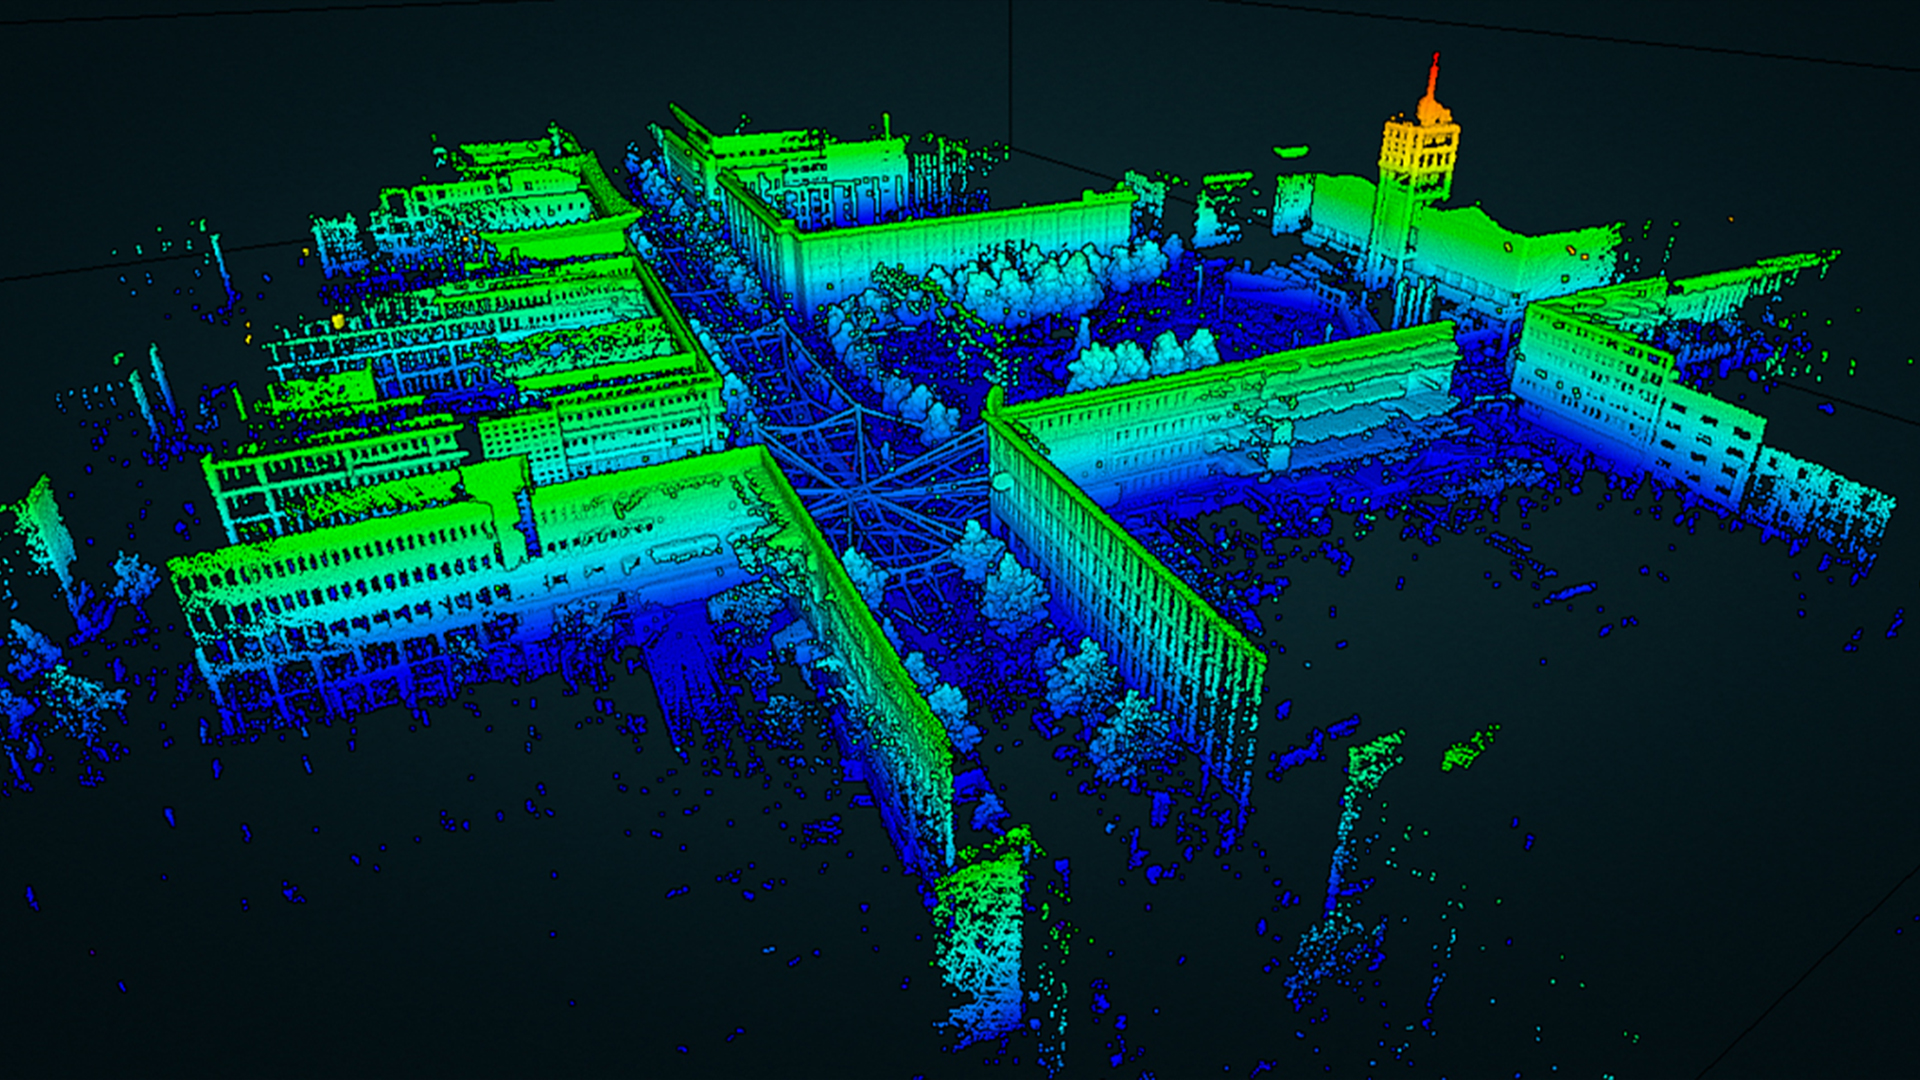
\includegraphics[height=3.25cm]{slam.jpg}\\[4pt]
      \textbf{Carte géométrique} $\rightarrow$ \alert{où} ?\\
      \legende{nuage de points, obstacles}
    \end{column}
    \begin{column}{0.48\textwidth}
      \centering
      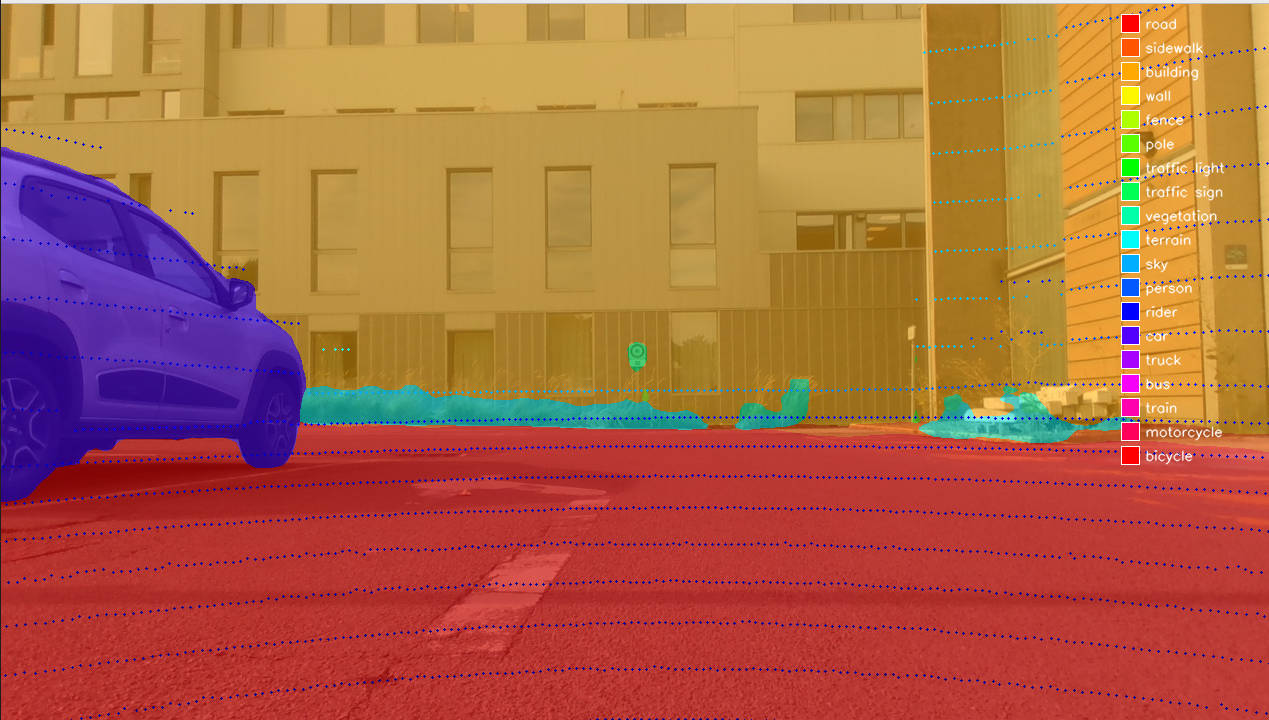
\includegraphics[height=3.25cm]{points.png}\\[4pt]
      \textbf{+ Sémantique} $\rightarrow$ \alert{quoi} ?\\
      \legende{route, bâtiment, végétation, véhicule\dots}
    \end{column}
  \end{columns}
  \vspace{0.3cm}
  \begin{tcolorbox}[question, width=\textwidth]
    Comment construire une carte \alert{sémantique}, \alert{partagée} entre robots,\\
    à partir du \alert{LiDAR} et de la \alert{caméra} ?
  \end{tcolorbox}
\end{frame}

% ----------------------------------------------------------------------
% À DIRE (~45 s)
%  - Démarche : deux briques existantes, complémentaires :
%      * LIO-SAM (LiDAR + IMU) : localisation précise du robot et carte
%        géométrique -> mais aucune information sémantique ;
%      * YOLO (caméra) : segmentation sémantique de l'image -> mais pas de
%        géométrie 3D.
%  - Mon travail = le framework ROS 2 qui les fusionne : chaque point
%    LiDAR reçoit un label YOLO, puis est placé dans le repère monde grâce
%    à la pose LIO -> carte sémantique 2D/3D exportée en GeoJSON.
%  - Puis trois extensions : prise en compte des loop closures, carte a
%    priori (OpenStreetMap), et passage au multi-robots.
%  - Validation : jeu de données KITTI, puis deux robots AgileX réels
%    (Scout Mini et Ranger).
% ----------------------------------------------------------------------
\begin{frame}{Objectifs et démarche}
  \centering
  \begin{tikzpicture}[font=\scriptsize]
    % Capteurs
    \node[capteur] (lidar) at (0,1.0)   {LiDAR 3D};
    \node[capteur] (imu)   at (0,0.05)  {IMU {\tiny(+ GPS)}};
    \node[capteur] (cam)   at (0,-1.25) {Caméra};
    % Briques existantes
    \node[boite=2.6cm, minimum height=0.95cm] (lio)  at (2.85,0.52)  {\textbf{LIO-SAM}\\ pose + carte géométrique};
    \node[boite=2.6cm, minimum height=0.95cm] (yolo) at (2.85,-1.25) {\textbf{YOLO}\\ segmentation sémantique};
    % Contribution
    \node[donnee=2.4cm, minimum height=1.2cm] (fus) at (6.0,-0.35) {\textbf{Fusion}\\ LiDAR -- caméra\\ {\tiny points 3D étiquetés}};
    \node[sortie=2.3cm, minimum height=1.2cm]  (carte) at (8.95,-0.35) {Carte sémantique\\ 2D / 3D\\ {\tiny\mdseries GeoJSON}};
    \node[boite=2.3cm, fill=softblue, minimum height=1.2cm] (multi) at (11.85,-0.35) {\textbf{Multi-robots}\\ carte commune};
    % Flèches
    \draw[fleche] (lidar.east) -- ++(0.3,0) |- (lio.west);
    \draw[fleche] (imu.east) -- ++(0.3,0) |- (lio.west);
    \draw[fleche] (cam) -- (yolo);
    \draw[fleche] (lidar.north) -- ++(0,0.35) -| node[pos=0.25, above, text=textgray, font=\tiny] {nuage de points} (fus.north);
    \draw[fleche] (lio.east) -- ++(0.35,0) |- (fus.west);
    \draw[fleche] (yolo.east) -- ++(0.35,0) |- (fus.west);
    \draw[fleche] (fus) -- (carte);
    \draw[fleche] (carte) -- (multi);
    % Ce qui existe / ce qui est développé
    \begin{scope}[on background layer]
      \node[groupe, fit=(lio)(yolo)] (existant) {};
      \node[groupe, draw=accent!70, fit=(fus)(carte)(multi)] (stage) {};
    \end{scope}
    \node[font=\tiny, text=textgray, anchor=north] at (existant.south) {briques existantes};
    \node[font=\tiny\bfseries, text=accent, anchor=north] at (stage.south) {développé pendant le stage};
  \end{tikzpicture}

  \vspace{0.45cm}
  {\small + \alert{loop closure} \quad\textbullet\quad + \alert{carte a priori} (OpenStreetMap)\\[3pt]
   Validation : \alert{KITTI} $\rightarrow$ robots réels \alert{Scout Mini} et \alert{Ranger}}
\end{frame}

% ======================================================================
%  PARTIE 2 -- LIO-SAM                                       (~3 min 15)
%  (pas d'état de l'art complet : uniquement ce qu'il faut pour
%   comprendre LIO-SAM et justifier son choix)
% ======================================================================
\section{LIO-SAM : SLAM LiDAR-inertiel}

% ----------------------------------------------------------------------
% À DIRE (~45 s)
%  - SLAM = localisation et cartographie simultanées : pour se localiser
%    il faut une carte, et pour faire une carte il faut savoir où l'on
%    est -> on estime les deux en même temps, avec les mêmes capteurs.
%  - Deux formulations :
%      * Online SLAM (filtres : EKF/UKF, filtre particulaire) : on n'estime
%        que la pose courante -> léger, temps réel, mais les erreurs
%        s'accumulent (dérive) sans correction possible du passé ;
%      * Full SLAM : on estime toute la trajectoire -> optimisation
%        globale, permet la fermeture de boucle (loop closure), qui
%        corrige rétroactivement toute la trajectoire. Plus coûteux.
%  - Le Full SLAM se représente par un graphe de facteurs : nœuds = poses
%    successives du robot (et amers), facteurs = contraintes issues des
%    mesures (odométrie, LiDAR...). Sous hypothèse de bruits gaussiens,
%    maximiser la probabilité a posteriori revient à minimiser une somme
%    d'erreurs quadratiques (moindres carrés), résolue efficacement par
%    GTSAM ou g2o.
%  - Figure : poses en bleu clair, amers en bleu foncé.
%  - Transition : LIO-SAM repose justement sur un graphe de facteurs.
% ----------------------------------------------------------------------
\begin{frame}{Prérequis : SLAM et graphe de facteurs}
  \begin{columns}[c]
    \begin{column}{0.5\textwidth}
      \textbf{SLAM} : se \alert{localiser} $\leftrightarrow$ \alert{cartographier}
      \vspace{0.25cm}
      \begin{itemize}
        \item \textbf{Online SLAM} -- filtres\\
              {\small $p(x_t, m \mid Z_t, U_t)$ : léger, mais \alert{dérive}}
        \item \textbf{Full SLAM} -- optimisation\\
              {\small $p(X_T, m \mid Z_T, U_T)$ : toute la trajectoire\\ $\Rightarrow$ \alert{loop closure} possible}
      \end{itemize}
      \vspace{0.3cm}
      \textbf{Graphe de facteurs}
      \begin{itemize}
        \item nœuds = \alert{poses} du robot
        \item facteurs = \alert{contraintes} capteurs
        \item moindres carrés : GTSAM, g2o
      \end{itemize}
    \end{column}
    \begin{column}{0.48\textwidth}
      \centering
      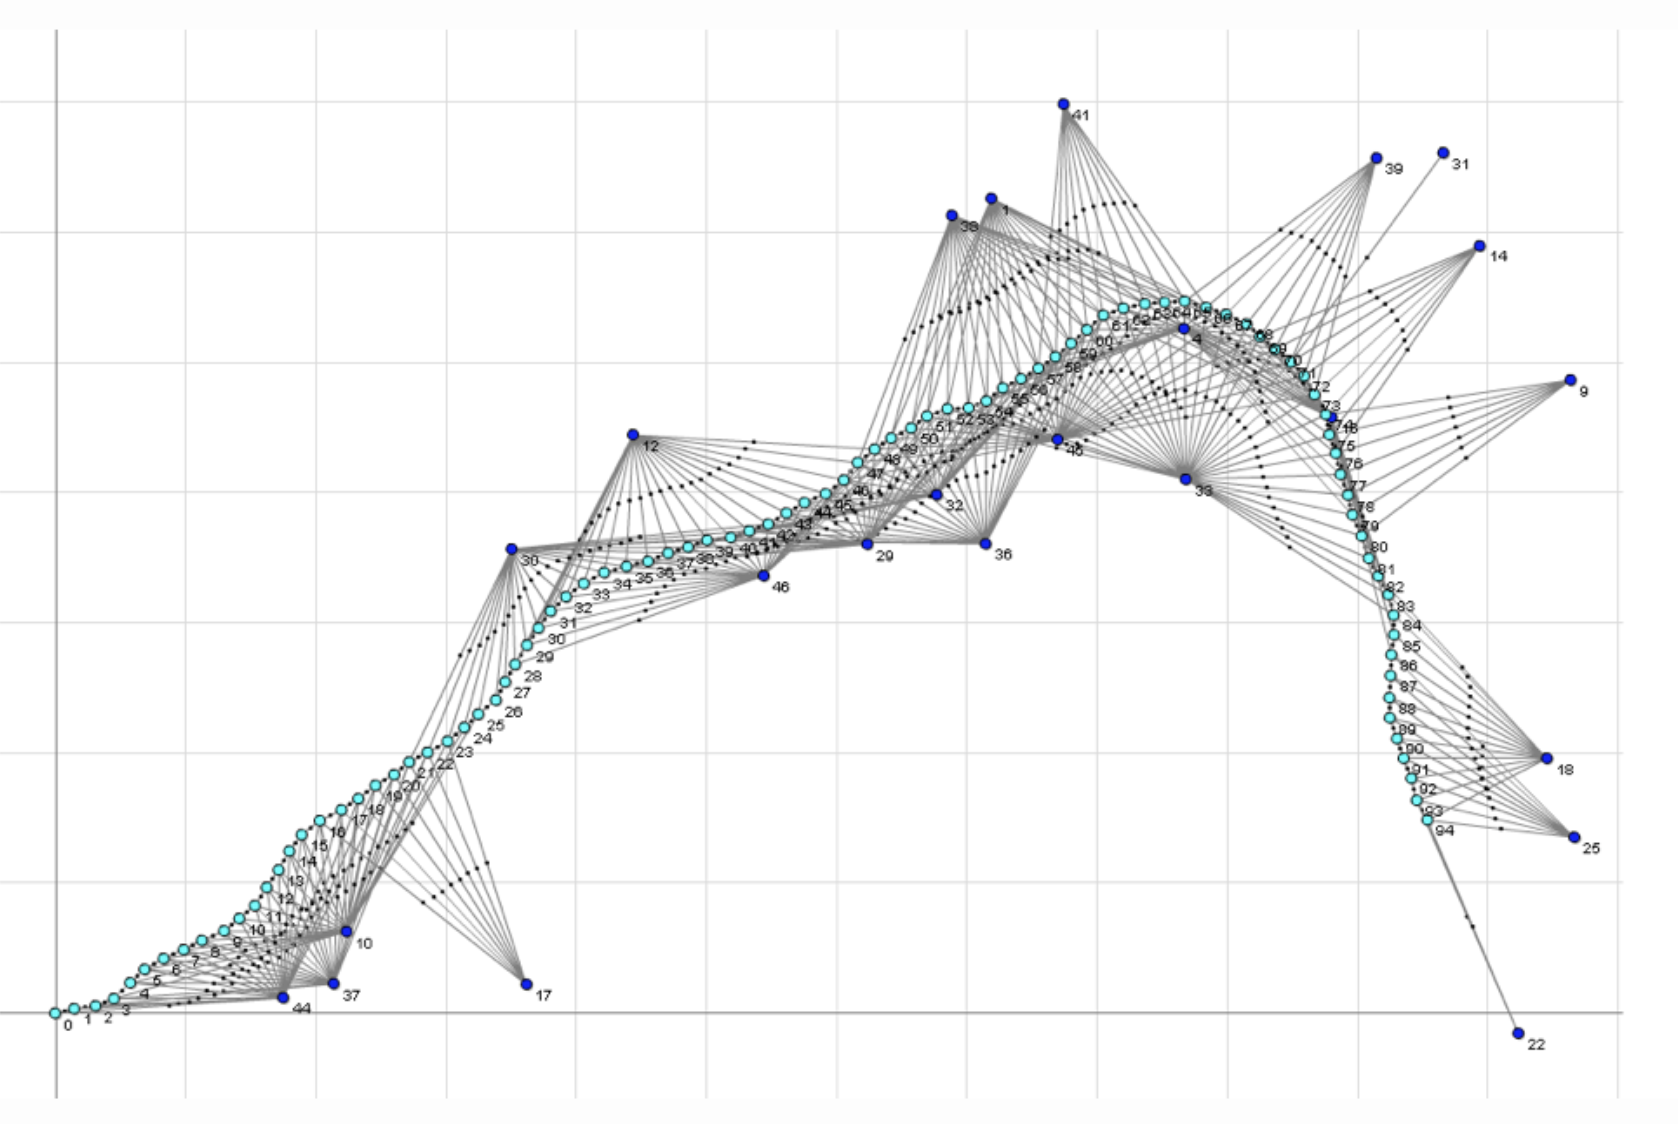
\includegraphics[width=\linewidth]{facteur.png}
      \legende{Exemple de graphe de facteurs (Dellaert, 2005)}
    \end{column}
  \end{columns}
\end{frame}

% ----------------------------------------------------------------------
% À DIRE (~1 min 15)
%  - LIO-SAM : LiDAR Inertial Odometry via Smoothing And Mapping
%    (Shan et al., IROS 2020).
%  - Entrées : LiDAR 3D + IMU 9 axes (+ GPS optionnel).
%    Sorties : odométrie haute fréquence, poses clés (keyframes) et carte
%    de points globale optimisée.
%  - Couplage SERRÉ LiDAR-IMU dans un graphe de facteurs (GTSAM) : les
%    nœuds x_i sont les états du robot, reliés par 4 types de facteurs :
%      1. Pré-intégration IMU (orange) : intègre les mesures IMU brutes
%         entre deux keyframes -> prédiction du mouvement à haute
%         fréquence ;
%      2. Odométrie LiDAR (vert) : recalage (scan matching) du scan
%         courant sur une carte locale construite avec les dernières
%         keyframes -> corrige la prédiction IMU ;
%      3. GPS (jaune), quand il est disponible : contrainte de position
%         absolue -> limite la dérive à long terme ;
%      4. Loop closure (noir) : relie deux états NON consécutifs (lieu
%         déjà visité, trouvé par recherche de proximité puis recalage)
%         -> corrige rétroactivement toute la trajectoire entre les deux.
%  - Les 3 premiers ne contraignent que des états voisins dans le temps ;
%    seule la loop closure corrige globalement.
% ----------------------------------------------------------------------
\begin{frame}{LIO-SAM : principe}
  \centering
  {\small \textbf{L}iDAR \textbf{I}nertial \textbf{O}dometry via \textbf{S}moothing \textbf{A}nd \textbf{M}apping
   \quad {\color{textgray}(Shan \emph{et al.}, IROS 2020)}\par}
  \vspace{0.2cm}
  \begin{tikzpicture}[font=\scriptsize]
    \node[capteur=3.3cm] (in) at (0,0) {\textbf{Entrées} : LiDAR 3D, IMU 9 axes, GPS {\tiny(option)}};
    \node[boite=3.9cm, draw=accent, thick] (gr) at (4.9,0) {\textbf{Graphe de facteurs} (GTSAM)\\ couplage \alert{serré} LiDAR -- IMU};
    \node[capteur=3.6cm] (out) at (9.9,0) {\textbf{Sorties} : odométrie haute fréquence, keyframes, carte globale};
    \draw[fleche] (in) -- (gr);
    \draw[fleche] (gr) -- (out);
  \end{tikzpicture}\par
  \vspace{0.15cm}
  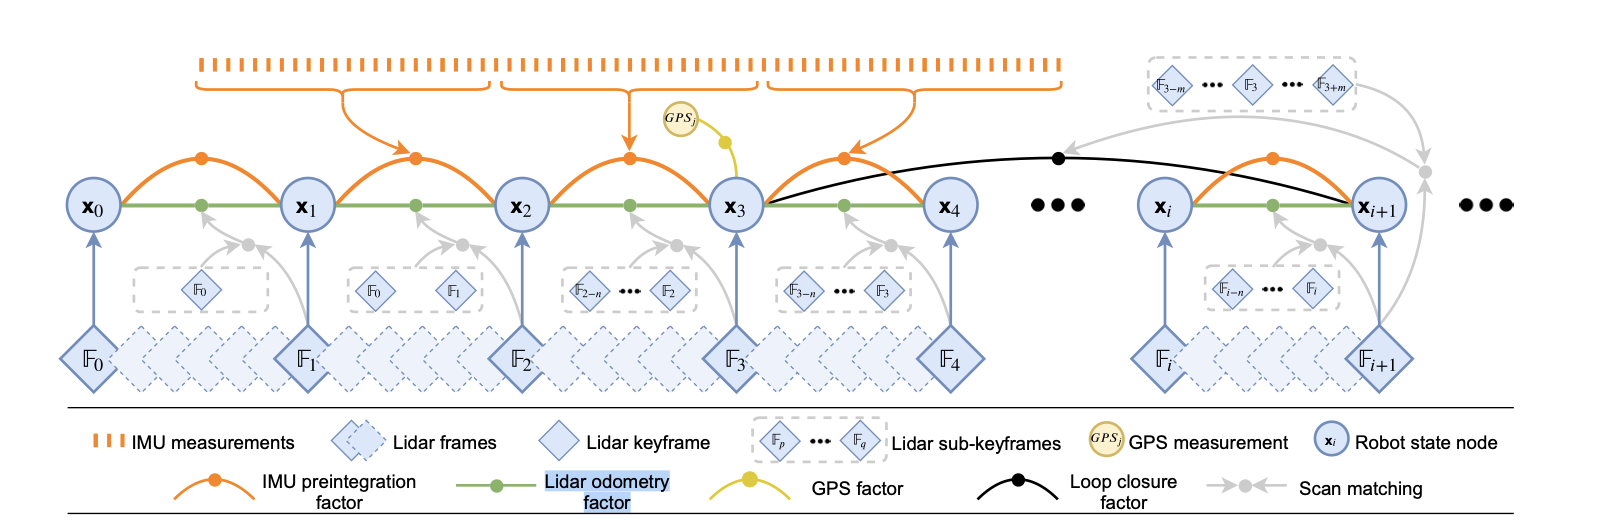
\includegraphics[width=0.84\textwidth]{liosam2.png}\par
  \vspace{0.1cm}
  \facteur{fIMU}{Pré-intégration IMU}{prédiction haute fréquence}\hfill
  \facteur{fLidar}{Odométrie LiDAR}{scan-matching, correction}\hfill
  \facteur{fGPS}{GPS}{position absolue}\hfill
  \facteur{fLoop}{Loop closure}{correction globale}
\end{frame}

% ----------------------------------------------------------------------
% À DIRE (~45 s)
%  - Côté logiciel, LIO-SAM = 4 nœuds ROS (de gauche à droite sur la
%    figure) qui s'échangent des messages :
%      1. imuPreintegration : reçoit l'IMU brute et publie une odométrie à
%         la fréquence de l'IMU (simple intégration), utilisée comme
%         prédiction par les autres nœuds ;
%      2. imageProjection : reçoit le nuage de points, l'IMU et cette
%         odométrie ; calcule une estimée initiale, organise le nuage et
%         corrige sa distorsion due au mouvement du robot pendant le scan
%         (deskewing) ; publie un message cloud_info ;
%      3. featureExtraction : extrait les points caractéristiques (arêtes
%         et plans, comme LOAM) et republie cloud_info ;
%      4. mapOptimization : recale le nuage sur la carte locale ->
%         odométrie LiDAR, puis optimise le graphe de facteurs (odométrie
%         LiDAR + GPS + loop closure) et publie l'odométrie optimisée.
%  - Cette odométrie optimisée repart vers imuPreintegration, qui
%    ré-estime le biais de l'IMU : cette boucle entre les nœuds = le
%    couplage serré de LIO-SAM.
%  - Pour mon framework : j'utilise la sortie odométrie de LIO (et plus
%    tard la trajectoire corrigée en cas de loop closure).
% ----------------------------------------------------------------------
\begin{frame}{LIO-SAM : architecture logicielle}
  \begin{columns}[c]
    \begin{column}{0.64\textwidth}
      \centering
      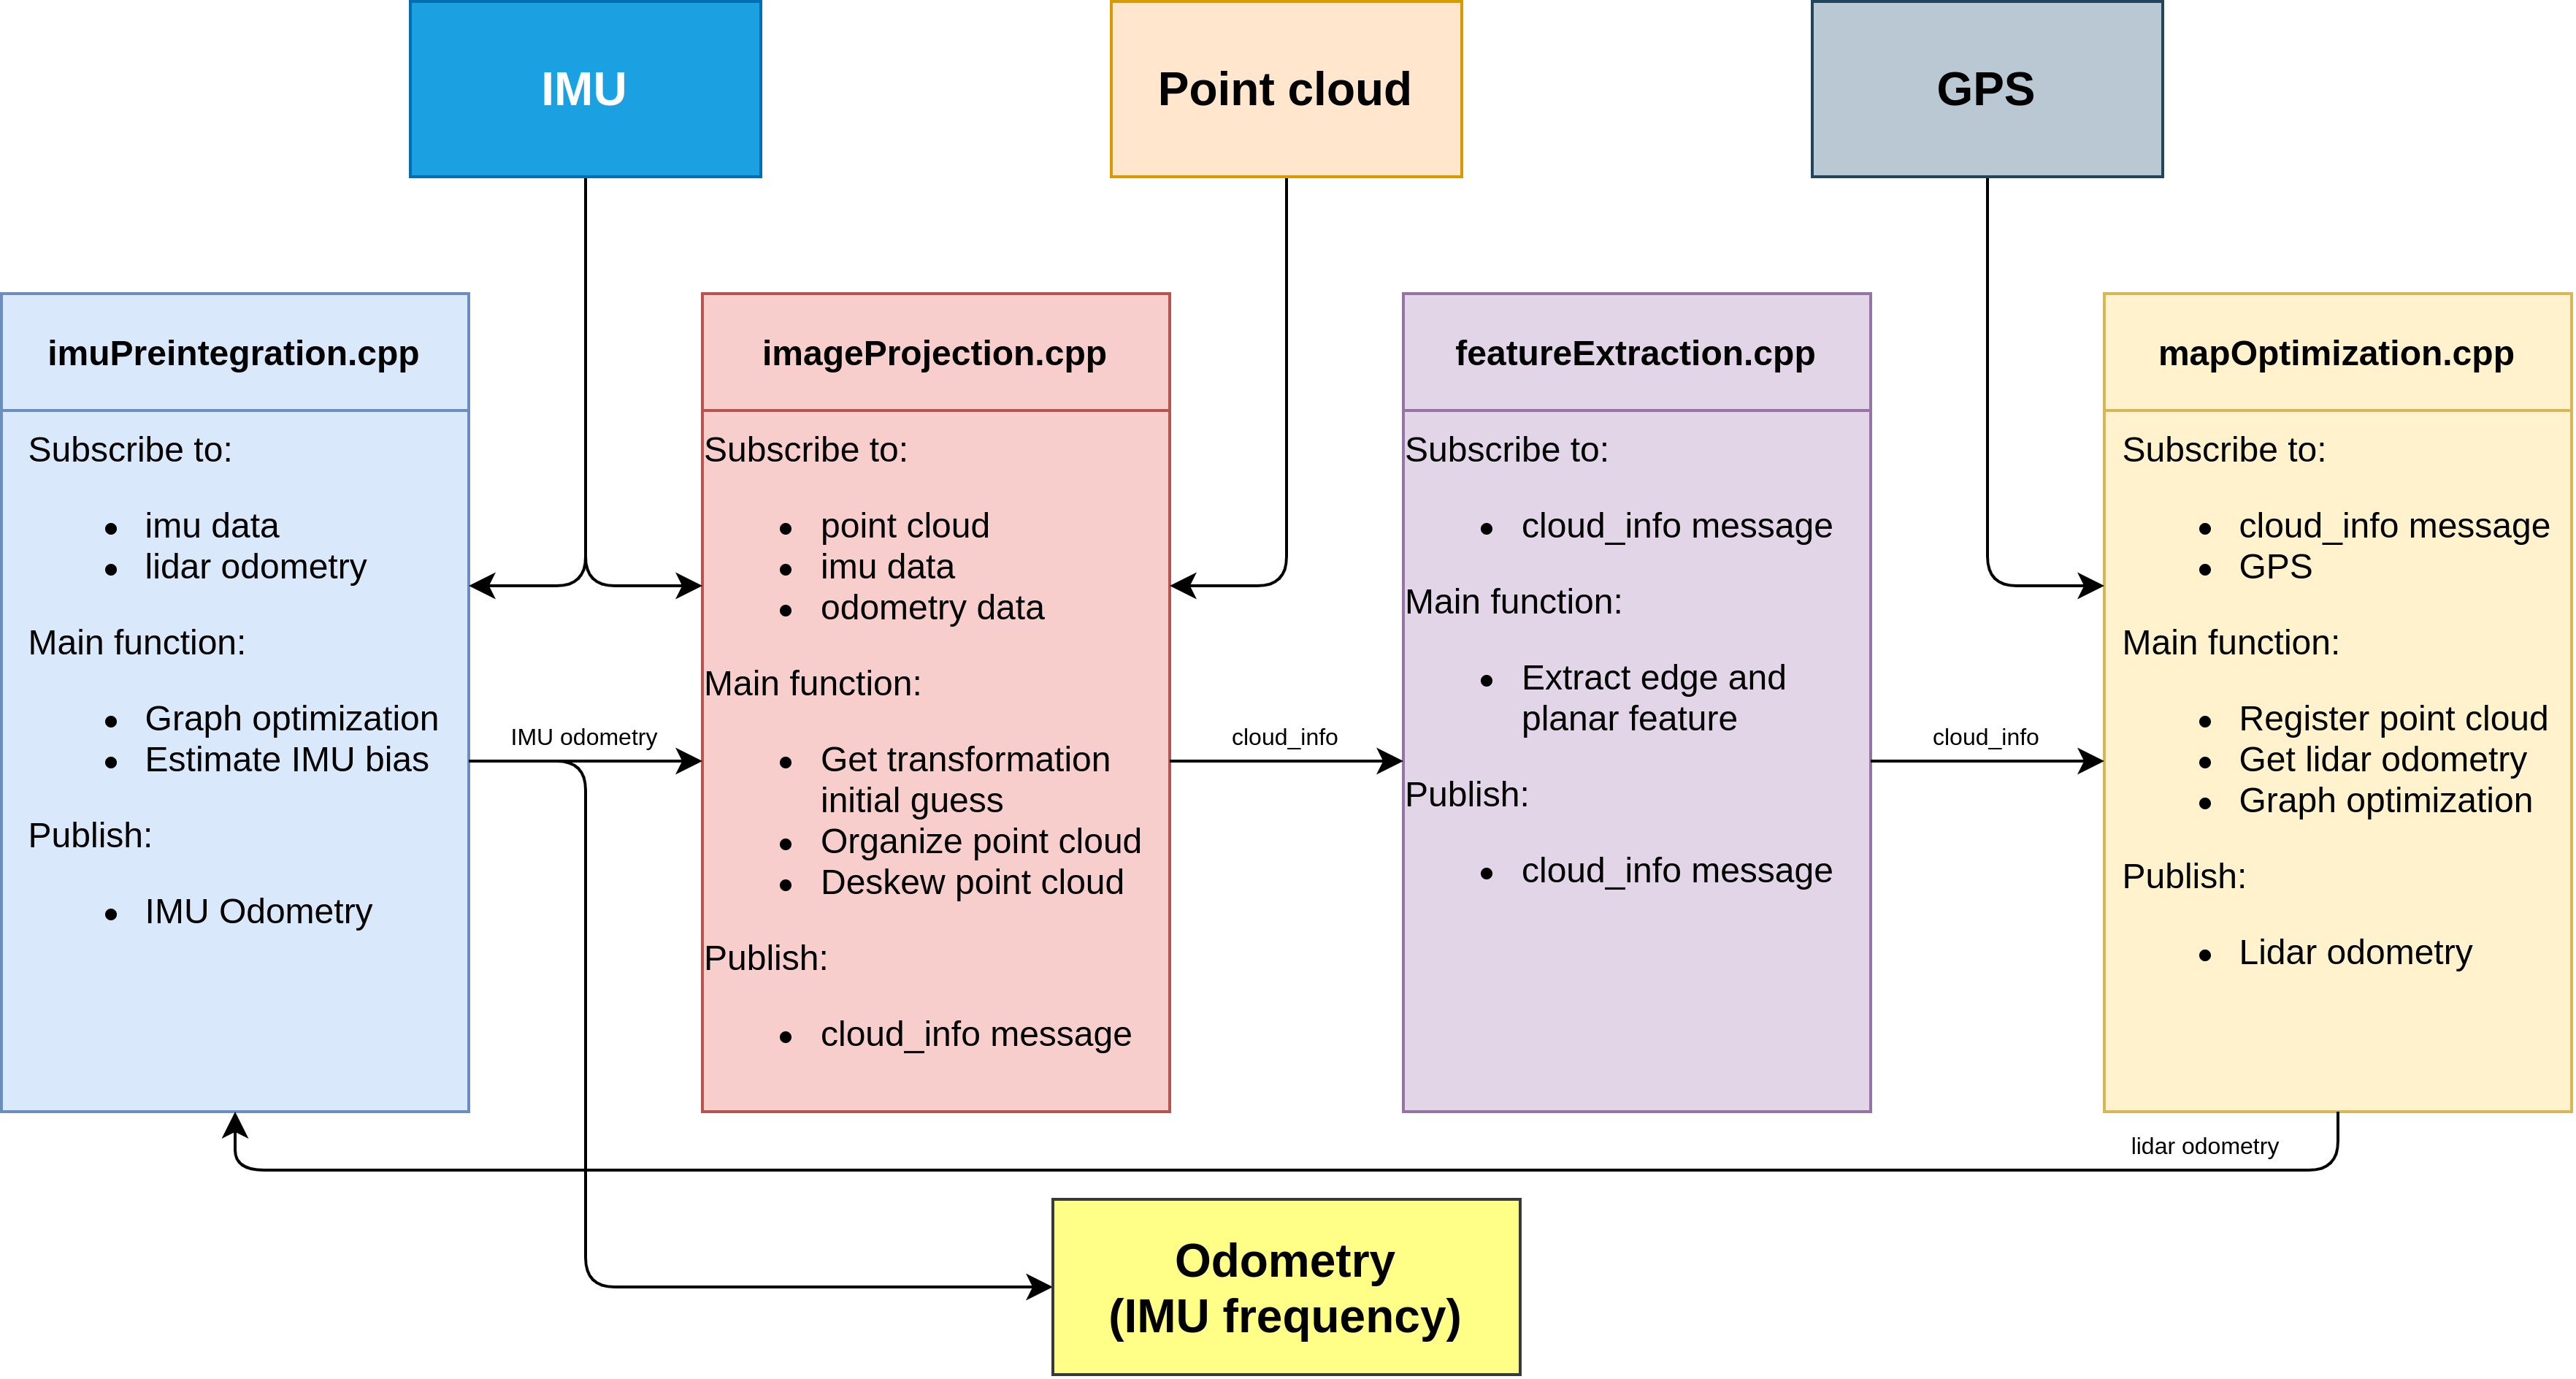
\includegraphics[width=\linewidth]{liosam.png}
      \legende{4 nœuds ROS et leurs messages (Shan \emph{et al.}, 2020)}
    \end{column}
    \begin{column}{0.34\textwidth}
      \small
      \begin{enumerate}
        \item \texttt{imuPreintegration}\\ {\footnotesize\color{textgray} odométrie IMU, \alert{biais IMU}}
        \item \texttt{imageProjection}\\ {\footnotesize\color{textgray} \alert{deskew} du nuage}
        \item \texttt{featureExtraction}\\ {\footnotesize\color{textgray} arêtes \& plans}
        \item \texttt{mapOptimization}\\ {\footnotesize\color{textgray} scan-matching + \alert{graphe}}
      \end{enumerate}
      \vspace{0.2cm}
      {\small $\circlearrowright$ odométrie LiDAR\\
      \phantom{$\circlearrowright$} $\rightarrow$ biais IMU\\[3pt]
      = couplage \alert{serré}\par}
    \end{column}
  \end{columns}
\end{frame}

% ----------------------------------------------------------------------
% À DIRE (~30 s)
%  - Pourquoi LIO-SAM : il exploite directement les capteurs des robots
%    (LiDAR 3D + IMU), il a une loop closure NATIVE (indispensable pour
%    corriger la dérive sur de longs trajets), et un portage ROS 2 mature.
%  - Surtout : le formalisme du graphe de facteurs est commun avec les
%    travaux du laboratoire (thèse de Clovis Adeler : diagnostic et
%    nouvelles contraintes GPS dans des architectures multi-robots) ->
%    base capable d'accueillir les futures briques du projet
%    (contraintes GPS multi-robots, planification, navigation).
%  - En pratique j'ai utilisé LIORF, une variante de LIO-SAM qui accepte
%    une IMU 6 axes (sans magnétomètre) : indispensable pour tester sur
%    KITTI, qui ne fournit pas de données magnétométriques.
%    Dans la suite je dis "LIO" pour LIO-SAM/LIORF.
%  - Si question : LIORF retire aussi le module d'extraction de
%    caractéristiques (cf. le titre du dépôt GitHub liorf).
%  - Si question sur les alternatives (état de l'art du rapport) :
%    FAST-LIO2 / Faster-LIO / DLIO / Point-LIO : très bons en odométrie
%    mais pas de loop closure native ; RTAB-Map : polyvalent mais plus
%    coûteux ; ORB-SLAM3 / VINS-Fusion : caméra seule, pas de LiDAR ;
%    SuMa++ : sémantique LiDAR mais académique, sans ROS 2 ni
%    multi-robots.
% ----------------------------------------------------------------------
\begin{frame}{Pourquoi LIO-SAM ?}
  \begin{columns}[c]
    \begin{column}{0.56\textwidth}
      \begin{itemize}
        \item[\ok] Capteurs des robots : \alert{LiDAR 3D + IMU}
        \item[\ok] \alert{Loop closure} native
        \item[\ok] Portage \alert{ROS 2} mature
        \item[\ok] \alert{Graphe de facteurs} : même formalisme\\ que les travaux du laboratoire
        \item[\ok] Base \alert{évolutive} pour ANR-SOS\\
              {\footnotesize\color{textgray} contraintes GPS multi-robots, navigation\dots}
      \end{itemize}
    \end{column}
    \begin{column}{0.38\textwidth}
      \begin{tcolorbox}[carte, title=En pratique : LIORF]
        Variante de LIO-SAM\\[4pt]
        \alert{IMU 6 axes}\\ {\footnotesize (sans magnétomètre)}\\[4pt]
        $\Rightarrow$ compatible \alert{KITTI}\\[6pt]
        {\footnotesize\color{textgray} dans la suite : « LIO »}
      \end{tcolorbox}
    \end{column}
  \end{columns}
\end{frame}

% ======================================================================
%  PARTIE 3 -- YOLO                                          (~1 min 30)
% ======================================================================
\section{YOLO : segmentation sémantique}

% ----------------------------------------------------------------------
% Schéma d'une scène simplifiée + points LiDAR, selon la tâche YOLO :
%   \scenesegm{1} = détection (boîtes), \scenesegm{2} = segmentation
%   d'instance, \scenesegm{3} = segmentation sémantique
% (\shorthandoff : les caractères ? : ! ; du français perturbent les calculs TikZ)
% ----------------------------------------------------------------------
\shorthandoff{;:!?}
\newcommand{\scenesegm}[1]{%
  \begin{tikzpicture}[x=0.95cm, y=0.95cm]
    \ifcase#1\or
      \def\sS{gray!8}\def\sB{gray!30}\def\sV{gray!22}\def\sR{gray!45}\def\sC{gray!62}%
    \or
      \def\sS{gray!8}\def\sB{gray!30}\def\sV{gray!22}\def\sR{gray!45}\def\sC{cVoiture!55}%
    \or
      \def\sS{cCiel!30}\def\sB{cBati!40}\def\sV{cVege!45}\def\sR{cRoute!45}\def\sC{cVoiture!55}%
    \fi
    \begin{scope}
      \clip (0,0) rectangle (4,2.4);
      \fill[\sS] (0,0) rectangle (4,2.4);                 % ciel
      \fill[\sB] (0,0.85) rectangle (1.5,2.0);            % bâtiment
      \fill[\sV] (3.3,1.35) ellipse (0.8 and 0.6);        % végétation
      \fill[\sR] (0,0) rectangle (4,0.85);                % route
      \fill[\sC, rounded corners=2pt] (1.6,0.25) rectangle (2.7,0.85);   % voiture
      \fill[\sC, rounded corners=2pt] (1.85,0.85) rectangle (2.45,1.15);
      \fill[black!70] (1.85,0.27) circle (0.12) (2.45,0.27) circle (0.12);
    \end{scope}
    \draw[gray!70] (0,0) rectangle (4,2.4);
    % Points LiDAR (pas de retour dans le ciel)
    \foreach \y in {0.12,0.37,0.62,0.87,1.12,1.37,1.62,1.87} {
      \foreach \x in {0.14,0.42,0.70,0.98,1.26,1.54,1.82,2.10,2.38,2.66,2.94,3.22,3.50,3.78} {
        % région du point : 1 voiture, 2 végétation, 3 bâtiment, 4 route, 0 ciel
        % (produits de booléens plutôt que && : la figure est dans un tableau)
        \pgfmathtruncatemacro{\sCar}{max((\x>=1.6)*(\x<=2.7)*(\y>=0.25)*(\y<=0.85),
                                         (\x>=1.85)*(\x<=2.45)*(\y>0.85)*(\y<=1.15))}%
        \pgfmathtruncatemacro{\sVeg}{((\x-3.3)/0.8)^2+((\y-1.35)/0.6)^2<=1}%
        \pgfmathtruncatemacro{\sBat}{(\x<=1.5)*(\y>0.85)*(\y<=2.0)}%
        \pgfmathtruncatemacro{\sRou}{\y<=0.85}%
        \pgfmathtruncatemacro{\sBoite}{(\x>=1.4)*(\x<=2.9)*(\y>=0.05)*(\y<=1.3)}%
        \def\sReg{0}%
        \ifnum\sRou=1 \def\sReg{4}\fi
        \ifnum\sBat=1 \def\sReg{3}\fi
        \ifnum\sVeg=1 \def\sReg{2}\fi
        \ifnum\sCar=1 \def\sReg{1}\fi
        \ifnum\sReg>0
          \def\sCoul{none}%
          \ifcase#1\or
            \ifnum\sBoite=1 \def\sCoul{cVoiture}\fi
          \or
            \ifnum\sReg=1 \def\sCoul{cVoiture}\fi
          \or
            \ifcase\sReg\or\def\sCoul{cVoiture}\or\def\sCoul{cVege}\or\def\sCoul{cBati}\or\def\sCoul{cRoute}\fi
          \fi
          \def\sAucune{none}%
          \ifx\sCoul\sAucune
            \filldraw[fill=white, draw=gray, line width=0.3pt] (\x,\y) circle (1.4pt);
          \else
            \filldraw[fill=\sCoul, draw=white, line width=0.3pt] (\x,\y) circle (1.6pt);
          \fi
        \fi
      }
    }
    \ifnum#1=1
      \draw[accent, very thick] (1.4,0.05) rectangle (2.9,1.3);
      \node[fill=accent, text=white, font=\tiny\bfseries, anchor=south west, inner sep=1.5pt] at (1.4,1.3) {car};
    \fi
  \end{tikzpicture}}
\shorthandon{;:!?}

% ----------------------------------------------------------------------
% À DIRE (~40 s)
%  - YOLO = You Only Look Once : réseau de neurones qui analyse l'image en
%    UNE SEULE passe, contrairement aux approches plus anciennes en deux
%    étapes (ex. famille R-CNN) qui repèrent d'abord des zones d'intérêt
%    puis les analysent une par une.
%  - Beaucoup plus rapide -> choix classique pour du temps réel embarqué
%    sur robot.
%  - Plusieurs versions (YOLOv5, v8, 11, 26), chacune plus précise et plus
%    rapide que la précédente ; et plusieurs tailles de modèle, de nano
%    (la plus légère, la moins précise) à extra-large (la plus lourde, la
%    plus précise).
%  - Choix : nano -> faible coût de calcul, car la chaîne de cartographie
%    (LIO) est déjà gourmande. Point de départ volontairement
%    conservateur : on pourra passer à small / medium selon la puissance
%    réellement disponible sur le robot.
% ----------------------------------------------------------------------
\begin{frame}{YOLO : principe}
  \begin{columns}[c]
    \begin{column}{0.36\textwidth}
      \begin{itemize}
        \item \alert{Y}ou \alert{O}nly \alert{L}ook \alert{O}nce
        \item Réseau de neurones :\\ \alert{une seule passe}
        \item \alert{Rapide} : temps réel,\\ embarqué sur robot
        \item Versions : v5, v8, 11, \alert{26}
      \end{itemize}
    \end{column}
    \begin{column}{0.62\textwidth}
      \centering
      \begin{tikzpicture}[font=\scriptsize]
        % Deux étapes
        \node[anchor=west, font=\scriptsize\bfseries, text=textgray] at (-0.6,1.85) {Approche en deux étapes};
        \node[capteur=1.0cm] (i1) at (0,1.2) {Image};
        \node[boite=1.55cm] (r1) at (1.9,1.2) {Zones d'intérêt};
        \node[boite=1.55cm] (c1) at (3.95,1.2) {Analyse une\\ par une};
        \node[boite=1.05cm] (o1) at (5.75,1.2) {Résultat};
        \draw[fleche] (i1) -- (r1);
        \draw[fleche] (r1) -- (c1);
        \draw[fleche] (c1) -- (o1);
        \node[right=1pt of o1, text=kored] {\ko\ lent};
        % YOLO
        \node[anchor=west, font=\scriptsize\bfseries, text=primaryblue] at (-0.6,0.35) {YOLO};
        \node[capteur=1.0cm] (i2) at (0,-0.3) {Image};
        \node[donnee=3.6cm] (c2) at (2.925,-0.3) {\textbf{un seul réseau, une seule passe}};
        \node[boite=1.05cm] (o2) at (5.75,-0.3) {Résultat};
        \draw[fleche] (i2) -- (c2);
        \draw[fleche] (c2) -- (o2);
        \node[right=1pt of o2, text=okgreen] {\ok\ rapide};
        % Tailles de modèle
        \node[anchor=west, font=\scriptsize\bfseries, text=textgray] at (-0.6,-1.25) {Tailles de modèle};
        \draw[thick, primaryblue!50] (0.2,-2.0) -- (6.2,-2.0);
        \foreach \px/\nom in {0.4/nano,1.8/small,3.2/medium,4.6/large,6.0/x-large} {
          \fill[primaryblue] (\px,-2.0) circle (2.2pt);
          \node[below=3pt, font=\scriptsize] at (\px,-2.0) {\nom};
        }
        \draw[accent, very thick] (0.4,-2.0) circle (5pt);
        \node[above=4pt, text=accent, font=\scriptsize\bfseries] at (0.4,-2.0) {choisi};
        \node[font=\tiny, text=textgray, anchor=north] at (0.4,-2.45) {rapide, léger};
        \node[font=\tiny, text=textgray, anchor=north] at (6.0,-2.45) {précis, lourd};
      \end{tikzpicture}
    \end{column}
  \end{columns}
\end{frame}

% ----------------------------------------------------------------------
% À DIRE (~50 s)
%  - Selon la tâche, YOLO donne :
%      * une boîte autour de chaque objet (détection) ;
%      * un masque de pixels par objet détecté (segmentation d'instance) ;
%      * un label pour CHAQUE pixel, fond compris (route, végétation,
%        ciel...) : segmentation sémantique (disponible avec YOLO26).
%  - Mon besoin : donner un label à chaque point LiDAR projeté dans
%    l'image.
%      * Avec une boîte : un point dans le coin de la boîte appartient en
%        fait au fond, mais il reçoit le label de l'objet -> erreurs.
%      * L'instance corrige ce problème pour les objets, mais ne masque
%        que les objets reconnus (véhicules, piétons...) : route,
%        végétation, sol restent sans label -> la plupart des points
%        n'auraient pas de label.
%      * La sémantique étiquette tous les pixels -> tous les points.
%  - Modèle retenu : YOLO26 nano en segmentation sémantique, entraîné sur
%    Cityscapes (scènes urbaines, 19 classes : route, trottoir, bâtiment,
%    végétation, voiture, piéton...).
% ----------------------------------------------------------------------
\begin{frame}{YOLO : pourquoi la segmentation \emph{sémantique} ?}
  \centering
  \begin{tabular}{@{}c@{\hspace{0.45cm}}c@{\hspace{0.45cm}}c@{}}
    \scenesegm{1} & \scenesegm{2} & \scenesegm{3} \\[2pt]
    \textbf{Détection} (boîtes) & \textbf{Segmentation d'instance} & \textbf{Segmentation sémantique} \\
    {\footnotesize \ko\ fond étiqueté « voiture »} &
    {\footnotesize \ko\ fond non étiqueté} &
    {\footnotesize \ok\ un label par pixel} \\
  \end{tabular}\par
  \vspace{0.25cm}
  \begin{tikzpicture}[font=\scriptsize]
    \filldraw[fill=cVoiture, draw=white] (0,0) circle (1.6pt); \node[right] at (0.05,0) {point LiDAR étiqueté};
    \filldraw[fill=white, draw=gray] (3.1,0) circle (1.4pt); \node[right] at (3.15,0) {point sans label};
  \end{tikzpicture}\par
  \vspace{0.25cm}
  \begin{tcolorbox}[question, width=0.78\textwidth]
    Modèle retenu : \alert{YOLO26 nano}, segmentation sémantique,
    entraîné sur \alert{Cityscapes} {\small(scènes urbaines, 19 classes)}
  \end{tcolorbox}
\end{frame}

% ======================================================================
%  PARTIE 4 -- Framework de fusion LiDAR-caméra              (~4 min)
% ======================================================================
\section{Framework de fusion LiDAR--caméra}

% ----------------------------------------------------------------------
% À DIRE (~50 s)
%  - C'est le cœur du travail : un framework ROS 2 qui combine la
%    localisation géométrique de LIO et la segmentation sémantique de
%    YOLO pour construire une carte sémantique.
%  - Deux parties bien distinctes (distinction qui sera essentielle pour
%    le multi-robots) :
%      1. Étiquetage des points, à chaque trame : synchronisation image /
%         LiDAR, projection des points LiDAR dans l'image, segmentation
%         YOLO, association d'un label à chaque point ; les trames
%         étiquetées sont mises en file d'attente.
%      2. Repère monde et carte : grâce à l'odométrie de LIO, chaque trame
%         est placée dans le repère monde, les points sont accumulés, puis
%         discrétisés en carte 2D / 3D exportée en GeoJSON.
%  - Objectif ANR-SOS : une brique embarquée, identique sur le Scout et
%    le Ranger (seules les calibrations changent).
% ----------------------------------------------------------------------
\begin{frame}{Architecture du nœud de fusion}
  \centering
  \begin{tikzpicture}[font=\scriptsize]
    % Partie 1 : étiquetage des points
    \node[capteur=1.5cm] (img)   at (0,1.95)    {Topic image};
    \node[capteur=1.5cm] (lid)   at (0,0.95)    {Topic LiDAR};
    \node[boite=2.1cm]   (sync)  at (2.35,1.45) {Synchronisation\\ temporelle};
    \node[boite=1.95cm]  (proj)  at (4.7,1.95)  {Projection\\ géométrique};
    \node[boite=1.95cm]  (yolo)  at (4.7,0.95)  {Segmentation\\ YOLO};
    \node[boite=1.85cm]  (assoc) at (7.0,1.45)  {Association\\ sémantique};
    \node[donnee=2.0cm]  (queue) at (9.3,1.45)  {File d'attente\\ {\tiny points + labels + t}};
    % Partie 2 : repère monde et carte
    \node[capteur=1.5cm] (odom)   at (0,-0.85)    {Topic\\ odométrie LIO};
    \node[boite=2.3cm]   (interp) at (4.7,-0.85)  {Historique +\\ interpolation de pose};
    \node[boite=2.0cm]   (monde)  at (9.3,-0.85)  {Transformation\\ repère monde};
    \node[sortie=2.1cm]  (carte)  at (11.8,-0.85) {Carte sémantique\\ {\tiny\mdseries 2D / 3D, GeoJSON}};
    % Flèches
    \draw[fleche] (img.east) -- ++(0.25,0) |- (sync.west);
    \draw[fleche] (lid.east) -- ++(0.25,0) |- (sync.west);
    \draw[fleche] (sync.east) -- ++(0.2,0) |- (proj.west);
    \draw[fleche] (sync.east) -- ++(0.2,0) |- (yolo.west);
    \draw[fleche] (proj.east) -- ++(0.2,0) |- (assoc.west);
    \draw[fleche] (yolo.east) -- ++(0.2,0) |- (assoc.west);
    \draw[fleche] (assoc) -- (queue);
    \draw[fleche] (queue) -- (monde);
    \draw[fleche] (odom) -- (interp);
    \draw[fleche] (interp) -- (monde);
    \draw[fleche] (monde) -- (carte);
    % Groupes
    \begin{scope}[on background layer]
      \node[groupe, fit=(img)(lid)(sync)(proj)(yolo)(assoc)(queue)] (g1) {};
      \node[groupe, draw=accent!70, fit=(odom)(interp)(monde)(carte)] (g2) {};
    \end{scope}
    \node[anchor=south west, font=\scriptsize\bfseries, text=primaryblue] at (g1.north west) {1. Étiquetage des points \mdseries(à chaque trame)};
    \node[anchor=north west, font=\scriptsize\bfseries, text=accent] at (g2.south west) {2. Repère monde et génération de la carte};
  \end{tikzpicture}
\end{frame}

% ----------------------------------------------------------------------
% À DIRE (~50 s)
%  - Synchronisation : les flux image et LiDAR n'arrivent ni au même
%    instant ni à la même fréquence -> ApproximateTimeSynchronizer
%    (message_filters) apparie les messages dont les horodatages sont
%    proches (écart max 50 ms). En plus, une fréquence cible : les paires
%    reçues trop tôt sont ignorées pour ne pas accumuler de retard.
%  - Projection en deux produits matriciels, en coordonnées homogènes :
%      * matrice extrinsèque [R|t] : du repère LiDAR au repère optique de
%        la caméra ; dépend du montage physique -> propre à chaque robot ;
%      * matrice intrinsèque K : paramètres internes de la caméra et
%        résolution (lue sur le topic camera_info).
%    -> pour chaque point : un pixel (u, v) et une profondeur z_c.
%    Les deux matrices sont déterminées une fois par robot et chargées en
%    paramètres au démarrage du nœud.
%  - Trois filtres : profondeur <= 0 (derrière la caméra), pixel hors de
%    l'image (hors champ de vision), distance > portée max (points
%    lointains, moins fiables pour l'association).
% ----------------------------------------------------------------------
\begin{frame}{Projection des points LiDAR dans l'image}
  \begin{columns}[c]
    \begin{column}{0.5\textwidth}
      \[
        z_c \begin{pmatrix} u\\ v\\ 1 \end{pmatrix}
        = \underbrace{K}_{\text{intrinsèque}}\;
          \underbrace{[\,R \mid t\,]}_{\text{extrinsèque}}
          \begin{pmatrix} X\\ Y\\ Z\\ 1 \end{pmatrix}_{\!\text{LiDAR}}
      \]
      \vspace{-0.1cm}
      \begin{itemize}
        \item $K$ : caméra {\footnotesize\color{textgray}(topic \texttt{camera\_info})}
        \item $[R \mid t]$ : LiDAR $\rightarrow$ caméra, \alert{propre à chaque robot}
        \item \textbf{3 filtres} : $z_c > 0$, \ $(u,v)$ dans l'image, \ distance $<$ portée max
        \item Synchronisation image / LiDAR\\
              {\footnotesize\color{textgray}\texttt{ApproximateTimeSynchronizer}, $\Delta t \leq 50$ ms}
      \end{itemize}
    \end{column}
    \begin{column}{0.48\textwidth}
      \centering
      \begin{tikzpicture}[font=\scriptsize]
        % champ de vision (demi-angle 24°) limité à la portée max (rayon 4,2)
        \fill[softblue] (0,0) -- (3.837,1.708) arc[start angle=24, end angle=-24, radius=4.2] -- cycle;
        \draw[primaryblue!40] (0,0) -- (3.837,1.708);
        \draw[primaryblue!40] (0,0) -- (3.837,-1.708);
        \draw[primaryblue!50, dashed] (3.837,1.708) arc[start angle=24, end angle=-24, radius=4.2];
        \node[text=textgray, font=\tiny, anchor=north] at (3.837,-1.75) {portée max};
        \draw[gray, dashed] (0,0) -- (4.55,0) node[right, font=\tiny] {$z_c$};
        % plan image
        \draw[very thick, primaryblue] (1,-0.445) -- (1,0.445);
        \node[text=primaryblue, font=\tiny, anchor=south] at (1,0.47) {image};
        % caméra et LiDAR
        \fill[primaryblue] (0,0) circle (2.2pt);
        \node[anchor=east, font=\scriptsize] at (-0.08,0.12) {caméra};
        \node[draw=primaryblue, fill=white, rounded corners=1pt, minimum width=0.5cm, minimum height=0.3cm] (L) at (-0.5,-1.35) {};
        \node[anchor=north, font=\scriptsize] at (L.south) {LiDAR};
        \draw[->, thick, accent] (L.north) -- node[left, font=\scriptsize] {$[R \mid t]$} (-0.05,-0.08);
        % point valide et sa projection sur le plan image
        \draw[accent, densely dotted, thick] (0,0) -- (3.1,0.8);
        \fill[accent] (3.1,0.8) circle (2.3pt) node[above right=-1pt] {\ok};
        \fill[accent] (1,0.258) circle (1.8pt);
        \node[anchor=south east, font=\tiny] at (0.97,0.27) {$(u,v)$};
        % points rejetés
        \fill[kored] (1.9,1.5) circle (2.2pt) node[right] {\ko\ hors image};
        \fill[kored] (4.45,-0.6) circle (2.2pt) node[below] {\ko\ trop loin};
        \fill[kored] (-0.9,0.75) circle (2.2pt) node[above] {\ko\ $z_c \leq 0$};
      \end{tikzpicture}
    \end{column}
  \end{columns}
\end{frame}

% ----------------------------------------------------------------------
% À DIRE (~30 s)
%  - En parallèle, l'image passe dans YOLO (nano, segmentation
%    sémantique) -> un masque qui associe une classe à chaque pixel.
%  - L'association consiste simplement à lire, pour chaque point LiDAR
%    valide, la valeur du masque au pixel (u, v), puis à convertir cet
%    identifiant en nom de classe.
%  - C'est ça, la fusion : chaque point garde sa position 3D précise
%    (LiDAR) et hérite d'un label sémantique (caméra).
%  - Affichage OpenCV en temps réel : masque sémantique superposé à
%    l'image + points LiDAR projetés (couleur selon la distance) +
%    légende des classes. Il ne sert pas au calcul de la carte, mais
%    permet de vérifier en direct la calibration et l'association.
% ----------------------------------------------------------------------
\begin{frame}{Association sémantique}
  \centering
  {\small pixel $(u,v)$ $\rightarrow$ label du masque YOLO
   \quad$\Rightarrow$\quad point = \alert{position 3D} (LiDAR) + \alert{label} (caméra)\par}
  \vspace{0.3cm}
  \begin{tabular}{@{}c@{\hspace{0.35cm}}c@{}}
    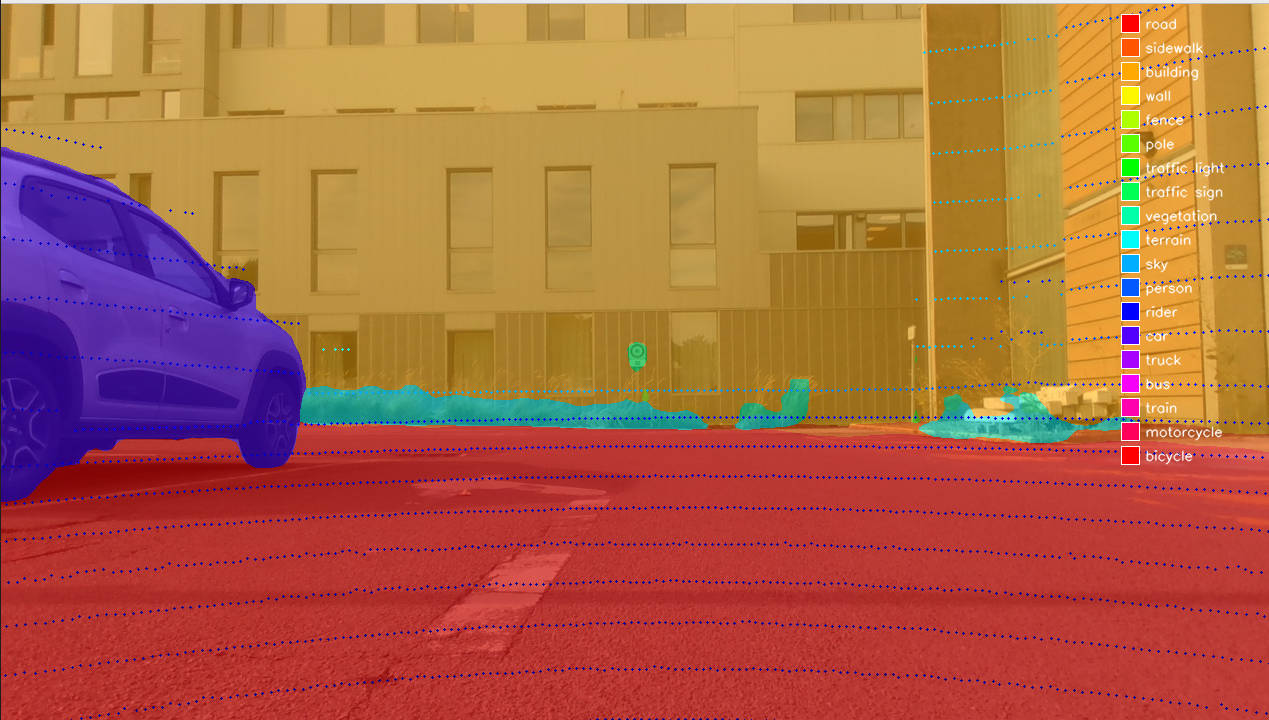
\includegraphics[height=3.9cm]{points.png} &
    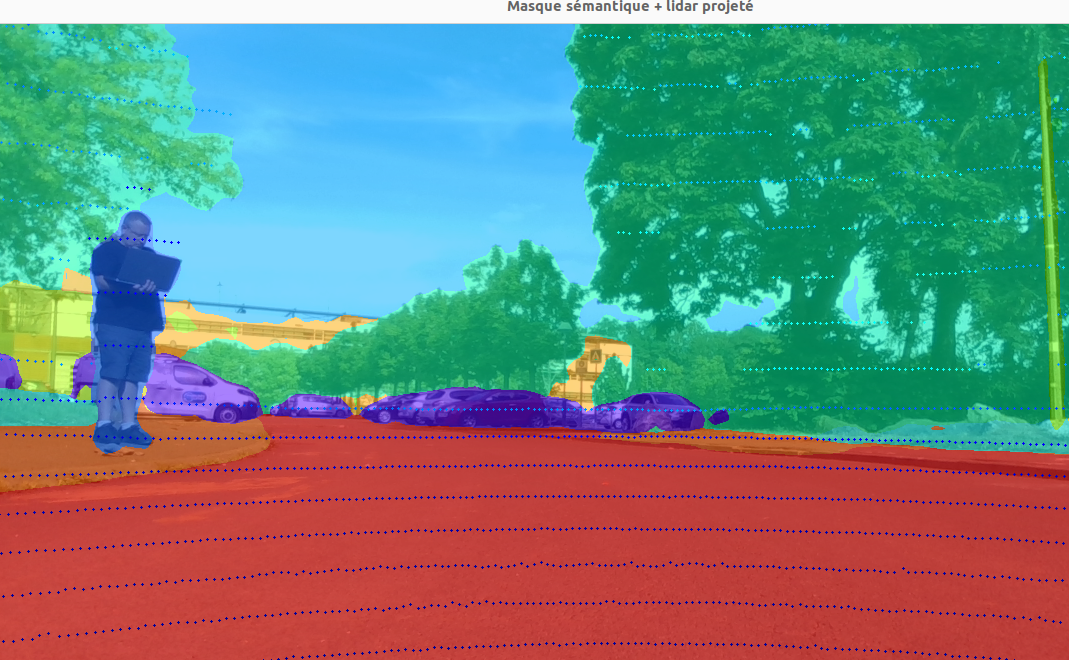
\includegraphics[height=3.9cm]{opencv_ranger.png} \\[1pt]
    \legende{Scout Mini -- parking du bâtiment ESPRIT} &
    \legende{Ranger} \\
  \end{tabular}\par
  \vspace{0.2cm}
  {\small Affichage \alert{OpenCV} temps réel : contrôle visuel de la \alert{calibration}\par}
\end{frame}

% ----------------------------------------------------------------------
% À DIRE (~50 s)
%  - Pour placer les points dans le repère monde, il faut la pose du
%    robot à l'instant exact de chaque trame.
%  - Deux options : l'arbre de transformations ROS (TF) ou le topic
%    d'odométrie de LIO. TF est plus coûteux (chaque recherche parcourt
%    l'arbre odom -> base_link -> lidar_link...) -> choix du topic
%    d'odométrie, et le nœud reconstitue lui-même la pose.
%  - L'odométrie arrive indépendamment des trames : on garde un
%    historique ; une trame n'est traitée que si l'historique couvre déjà
%    son horodatage, sinon elle attend dans une file d'attente bornée
%    (ordre temporel garanti, mémoire maîtrisée).
%  - Interpolation entre les deux odométries qui encadrent la trame :
%    linéaire pour la position, sphérique (slerp) pour l'orientation
%    (quaternion), avec SciPy. La pose obtenue transforme les points du
%    repère LiDAR vers le repère monde.
% ----------------------------------------------------------------------
\begin{frame}{Passage dans le repère monde}
  \begin{columns}[c]
    \begin{column}{0.45\textwidth}
      \begin{itemize}
        \item Pose du robot à l'instant \alert{exact} de chaque trame
        \item TF {\footnotesize(coûteux)} $\rightarrow$ \alert{topic odométrie} de LIO
        \item Historique des odométries\\ + \alert{file d'attente} bornée
        \item Interpolation :\\ \alert{lerp} (position), \alert{slerp} (orientation)
      \end{itemize}
      \vspace{0.15cm}
      \centering
      $P_{\text{monde}} = R(t)\,P_{\text{LiDAR}} + T(t)$
    \end{column}
    \begin{column}{0.53\textwidth}
      \centering
      \begin{tikzpicture}[font=\scriptsize]
        \draw[->, thick, primaryblue!70] (-0.2,0) -- (6.4,0) node[right] {$t$};
        % odométries LIO
        \foreach \px in {0.3,1.5,2.7,3.9} {
          \draw[primaryblue!35] (\px,0) -- (\px,0.5);
          \node[diamond, fill=primaryblue, inner sep=1.7pt] at (\px,0.5) {};
        }
        % trames LiDAR + caméra
        \foreach \px in {0.9,2.2,3.4} {
          \draw[accent!40] (\px,0) -- (\px,-0.5);
          \fill[accent] (\px,-0.5) circle (3pt);
        }
        \draw[accent!40] (5.0,0) -- (5.0,-0.5);
        \filldraw[fill=white, draw=accent, thick] (5.0,-0.5) circle (3pt);
        \node[below=3pt, text=accent, align=center] at (5.0,-0.5) {en attente\\ {\tiny(pas encore d'odométrie)}};
        % interpolation de la trame en t
        \node[above=3pt] at (1.5,0.5) {$t_0$};
        \node[above=3pt] at (2.7,0.5) {$t_1$};
        \node[below=3pt] at (2.2,-0.5) {$t$};
        \draw[accent, thick, ->] (1.55,0.62) to[bend left=35] (2.12,-0.38);
        \draw[accent, thick, ->] (2.65,0.62) to[bend right=35] (2.28,-0.38);
        % légende
        \node[diamond, fill=primaryblue, inner sep=1.7pt] at (0.3,-1.75) {};
        \node[anchor=west] at (0.45,-1.75) {odométrie LIO};
        \fill[accent] (3.0,-1.75) circle (3pt);
        \node[anchor=west] at (3.15,-1.75) {trame LiDAR + caméra};
      \end{tikzpicture}\par
      \vspace{0.25cm}
      {\small
      $\alpha = \dfrac{t - t_0}{t_1 - t_0}$ \qquad
      $\mathbf{p}(t) = (1-\alpha)\,\mathbf{p}_0 + \alpha\,\mathbf{p}_1$\\[4pt]
      $q(t) = \operatorname{slerp}(q_0, q_1, \alpha)$\par}
    \end{column}
  \end{columns}
\end{frame}

% ----------------------------------------------------------------------
% À DIRE (~50 s)
%  - Une fois les points accumulés dans le repère monde, des fonctions
%    "hors ligne" (déclenchées à l'arrêt du nœud) les transforment en
%    carte exploitable. En multi-robots, elles tourneront périodiquement.
%  - Carte 2D : grille de cases carrées (GeoPandas). Pour chaque case :
%    le label dominant (le plus représenté parmi les points de la case),
%    le pourcentage de points qui portent ce label (indicateur de
%    confiance) et le temps d'acquisition (min et max).
%  - Carte 3D : même principe avec des voxels, indexés par trois indices
%    entiers calculés à partir de la position et du pas en x, y, z.
%  - Deux informations en plus :
%      * une confiance liée à la portée : un point mesuré près du LiDAR
%        est plus fiable qu'un point mesuré à la portée max ;
%      * un indice de traversabilité déduit du label dominant (table de
%        correspondance, ex. route = très traversable) -- encore limitée
%        à quelques labels ; piste : ajouter l'élévation.
%  - Export GeoJSON : une case (ou un voxel) = une entité, avec son
%    centre, son label et ses indicateurs.
% ----------------------------------------------------------------------
\begin{frame}{Génération de la carte sémantique}
  \begin{columns}[c]
    \begin{column}{0.5\textwidth}
      \centering
      \begin{tikzpicture}[font=\scriptsize]
        % points étiquetés dans la grille
        \foreach \px/\py/\coul in {
            0.17/1.87/cVege, 0.53/1.91/cVege, 0.36/2.13/cVege, 0.17/2.37/cBati, 0.56/2.36/cVege,
            1.02/1.87/cBati, 1.38/1.91/cBati, 1.21/2.13/cVege, 1.02/2.37/cBati, 1.41/2.36/cBati,
            1.87/1.87/cBati, 2.23/1.91/cBati, 2.06/2.13/cBati, 1.87/2.37/cAutre, 2.26/2.36/cBati,
            0.17/1.02/cRoute, 0.53/1.06/cRoute, 0.36/1.28/cAutre, 0.17/1.52/cRoute, 0.56/1.51/cRoute,
            1.02/1.02/cRoute, 1.38/1.06/cRoute, 1.21/1.28/cRoute, 1.02/1.52/cRoute, 1.41/1.51/cAutre,
            1.87/1.02/cAutre, 2.23/1.06/cAutre, 2.06/1.28/cRoute, 1.87/1.52/cAutre, 2.26/1.51/cBati,
            0.17/0.17/cRoute, 0.53/0.21/cRoute, 0.36/0.43/cRoute, 0.17/0.67/cRoute, 0.56/0.66/cRoute,
            1.02/0.17/cRoute, 1.38/0.21/cAutre, 1.21/0.43/cRoute, 1.02/0.67/cRoute, 1.41/0.66/cRoute,
            1.87/0.17/cAutre, 2.23/0.21/cAutre, 2.06/0.43/cAutre, 1.87/0.67/cRoute, 2.26/0.66/cAutre} {
          \fill[\coul] (\px,\py) circle (2pt);
        }
        \draw[step=0.85, gray!60] (0,0) grid (2.55,2.55);
        \node[anchor=north] at (1.275,-0.1) {points étiquetés};
        % flèche
        \draw[fleche] (2.8,1.275) -- node[above, align=center] {label\\ dominant} (3.9,1.275);
        % cases agrégées
        \begin{scope}[xshift=4.15cm]
          \foreach \ci/\cj/\coul in {0/2/cVege, 1/2/cBati, 2/2/cBati,
                                0/1/cRoute, 1/1/cRoute, 2/1/cAutre,
                                0/0/cRoute, 1/0/cRoute, 2/0/cAutre} {
            \fill[\coul!75] (\ci*0.85,\cj*0.85) rectangle ++(0.85,0.85);
          }
          \draw[step=0.85, white, thick] (0,0) grid (2.55,2.55);
          \node[text=white, font=\scriptsize\bfseries] at (1.275,1.275) {80\,\%};
          \node[anchor=north] at (1.275,-0.1) {cases (ou voxels)};
        \end{scope}
        % légende des classes
        \foreach \coul/\nom [count=\k] in {cRoute/route, cBati/bâtiment, cVege/végétation, cAutre/autre} {
          \fill[\coul] ({(\k-1)*1.7},-1.0) rectangle ++(0.25,0.25);
          \node[anchor=west, font=\tiny] at ({(\k-1)*1.7+0.3},-0.875) {\nom};
        }
      \end{tikzpicture}
    \end{column}
    \begin{column}{0.47\textwidth}
      \begin{itemize}
        \item Grille \alert{2D} ou voxels \alert{3D}
        \item Par case : \alert{label dominant}\\
              {\footnotesize\color{textgray} + \% (confiance), temps min/max}
        \item Confiance $\searrow$ avec la \alert{distance}
        \item \alert{Traversabilité}\\
              {\footnotesize\color{textgray} table label $\rightarrow$ valeur}
        \item Export \alert{GeoJSON}\\
              {\footnotesize\color{textgray} 1 case = 1 entité}
      \end{itemize}
    \end{column}
  \end{columns}
\end{frame}

% ======================================================================
%  PARTIE 5 -- Loop closure, carte a priori, multi-robots    (~3 min 10)
% ======================================================================
\section{Loop closure, carte a priori et multi-robots}

% ----------------------------------------------------------------------
% À DIRE (~40 s)
%  - Rappel : une loop closure = reconnaître qu'on repasse par un endroit
%    déjà visité, pour corriger la dérive accumulée sur TOUTE la
%    trajectoire (pas seulement la partie récente).
%  - La détection n'est pas faite par mon framework mais par LIO, qui
%    publie ensuite ses résultats (contraintes + trajectoire corrigée).
%  - Principe dans LIO :
%      1. à chaque nouvelle keyframe, recherche par arbre 3D (kd-tree)
%         des keyframes proches dans l'espace (rayon 15 m par défaut) ;
%      2. on écarte celles trop proches dans le temps (< 30 s), pour ne
%         pas "boucler" sur la trajectoire d'il y a quelques instants ;
%      3. sous-cartes de 25 keyframes voisines autour de la pose courante
%         et autour de la candidate, recalées par ICP ;
%      4. si le score ICP passe sous le seuil (0,3) -> nouvelle contrainte
%         dans le graphe -> optimisation globale.
%  - Réglage = compromis : rayon trop grand / seuil trop permissif ->
%    fausses boucles ; trop strict -> vraies boucles manquées.
%    (Tableau des paramètres en annexe.)
% ----------------------------------------------------------------------
\begin{frame}{Loop closure : détection par LIO}
  \begin{columns}[c]
    \begin{column}{0.42\textwidth}
      \centering
      \begin{tikzpicture}[font=\scriptsize, scale=1.25]
        % trajectoire estimée (avec dérive)
        \draw[primaryblue, thick] plot[smooth, tension=0.6] coordinates
          {(0,0) (1.2,-0.35) (2.6,-0.2) (3.4,0.6) (3.3,1.8) (2.2,2.5) (0.9,2.3) (0.15,1.5) (0.35,0.62)};
        \foreach \px/\py in {1.2/-0.35, 2.6/-0.2, 3.4/0.6, 3.3/1.8, 2.2/2.5, 0.9/2.3} {
          \filldraw[fill=white, draw=primaryblue] (\px,\py) circle (2.2pt);
        }
        % rayon de recherche autour de la pose courante
        \draw[accent, dashed] (0.35,0.62) circle (1.0);
        % keyframe récente, écartée
        \filldraw[fill=gray!30, draw=gray] (0.15,1.5) circle (2.2pt);
        \node[anchor=east, text=textgray, font=\tiny] at (0.05,1.55) {trop récente \ko};
        % keyframe candidate (départ) et pose courante
        \filldraw[fill=primaryblue, draw=primaryblue] (0,0) circle (2.8pt);
        \node[anchor=north east, font=\tiny] at (-0.05,-0.05) {départ};
        \filldraw[fill=accent, draw=accent] (0.35,0.62) circle (2.8pt);
        \node[anchor=west, text=accent, font=\tiny\bfseries] at (0.5,0.75) {pose courante};
        % contrainte de boucle
        \draw[fLoop, very thick] (0.35,0.62) to[bend left=45] node[right=1pt, font=\tiny] {ICP} (0,0);
        \draw[accent, thin] (0.35,0.62) -- (1.216,0.12);
        \node[text=accent, font=\tiny, anchor=north west] at (1.1,0.22) {15 m};
      \end{tikzpicture}
    \end{column}
    \begin{column}{0.56\textwidth}
      \begin{enumerate}
        \item Nouvelle keyframe $\rightarrow$ recherche \alert{kd-tree}\\
              {\footnotesize\color{textgray} keyframes proches dans l'espace (15 m)}
        \item On écarte les keyframes \alert{trop récentes}\\
              {\footnotesize\color{textgray} écart temporel $<$ 30 s}
        \item Sous-cartes ($\pm$ 25 keyframes) $\rightarrow$ recalage \alert{ICP}
        \item Score ICP $<$ 0,3 $\rightarrow$ \alert{nouveau facteur}\\
              {\footnotesize\color{textgray} optimisation globale du graphe}
      \end{enumerate}
    \end{column}
  \end{columns}
\end{frame}

% ----------------------------------------------------------------------
% À DIRE (~50 s)
%  - LIO corrige sa trajectoire, mais les points déjà placés dans ma
%    carte sémantique, eux, ne bougent pas -> il faut répercuter la
%    correction.
%  - Deux abonnements en plus : les contraintes de loop closure publiées
%    par LIO, et la trajectoire complète corrigée (topic path).
%  - Détection : dès que le nombre de contraintes publiées augmente, une
%    nouvelle boucle vient d'être intégrée par LIO.
%  - Toutes les trames traitées depuis le début sont conservées sous
%    forme brute (points filtrés + labels, avant passage au repère monde)
%    dans un second stockage (pending_frames_until_loop).
%  - Recalcul complet : chaque trame est retransformée dans le repère
%    monde avec la trajectoire CORRIGÉE, interpolée de la même façon
%    (lerp / slerp) -- interpolation d'autant plus nécessaire que la
%    trajectoire corrigée ne contient que les keyframes. Le nouveau nuage
%    remplace entièrement l'ancien. Le traitement courant continue en
%    parallèle.
%  - Test sur KITTI (loop closure forcée en réduisant le délai minimal,
%    car le bag ne fait pas une vraie boucle) : ça fonctionne, mais on
%    voit des trous = trames perdues. Le recalcul coûte de plus en plus
%    cher avec le temps, et la voiture dépasse 50 km/h sur la ligne
%    droite (les pertes commencent exactement là).
%  - Conclusion : limiter la vitesse des robots et le délai avant
%    transfert de la carte.
% ----------------------------------------------------------------------
\begin{frame}{Loop closure : mise à jour de la carte}
  \begin{columns}[c]
    \begin{column}{0.44\textwidth}
      \centering
      \begin{tikzpicture}[font=\scriptsize, node distance=0.42cm]
        \node[capteur=4.4cm] (b1) {LIO : nouvelle contrainte de boucle\\ {\tiny(nombre de contraintes $\nearrow$)}};
        \node[capteur=4.4cm, below=of b1] (b2) {Trajectoire \alert{corrigée} {\tiny(topic \texttt{path}, keyframes)}};
        \node[boite=4.4cm, below=of b2] (b3) {Ré-interpolation de \alert{toutes} les trames stockées\\ {\tiny\texttt{pending\_frames\_until\_loop}}};
        \node[sortie=4.4cm, below=of b3] (b4) {Nouveau nuage $\rightarrow$ remplace l'ancien};
        \draw[fleche] (b1) -- (b2);
        \draw[fleche] (b2) -- (b3);
        \draw[fleche] (b3) -- (b4);
      \end{tikzpicture}
    \end{column}
    \begin{column}{0.54\textwidth}
      \centering
      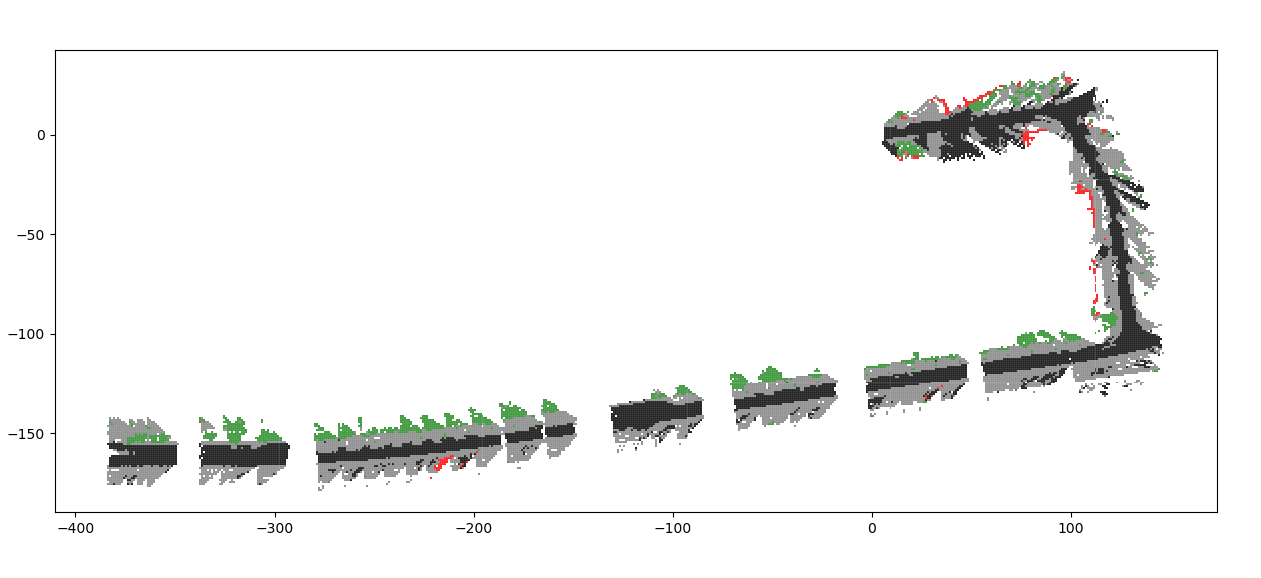
\includegraphics[width=\linewidth]{loop_kitti.png}
      \legende{KITTI, loop closure forcée : les trous = trames perdues}
      \vspace{0.25cm}
      {\small \ko\ recalcul de plus en plus \alert{coûteux}\\
       \ko\ vitesse $>$ 50 km/h $\rightarrow$ \alert{pertes}\par}
    \end{column}
  \end{columns}
\end{frame}

% ----------------------------------------------------------------------
% À DIRE (~50 s)
%  - Carte a priori = carte du terrain construite EN AMONT à partir de
%    données existantes (OpenStreetMap), pas par le robot.
%  - Deux rôles : référence de navigation disponible dès le démarrage, et
%    vérité terrain pour évaluer la carte sémantique produite par le
%    robot. À terme : réintégrée dans la cartographie elle-même.
%  - Construction : extraction de la zone via Overpass Turbo au format
%    GeoJSON, puis discrétisation en grille (GeoPandas, jointure spatiale
%    sjoin entre la grille et les polygones OSM).
%  - Problème : une case à cheval sur deux polygones (ex. bâtiment +
%    forêt) donne deux entrées. Solution : pas de discrétisation fin
%    (possible car la carte n'est chargée qu'une fois) + priorité entre
%    labels (un obstacle "bâtiment" l'emporte sur une zone libre) ; les
%    tags OSM sont aussi normalisés (ex. building=yes -> building).
%  - Intégration dans le nœud : coordonnées Lambert-93 ramenées dans un
%    repère local (on soustrait l'origine), puis position et cap initiaux
%    du robot (rotation + décalage) pour superposer les deux cartes.
%  - Limites : pas d'élévation ; pour l'instant, la carte a priori sert
%    de fond de carte, elle n'est pas fusionnée dans le GeoJSON produit.
% ----------------------------------------------------------------------
\begin{frame}{Carte a priori (OpenStreetMap)}
  \begin{columns}[c]
    \begin{column}{0.56\textwidth}
      \centering
      \begin{tikzpicture}
        \node[inner sep=0pt] (z) at (0,0) {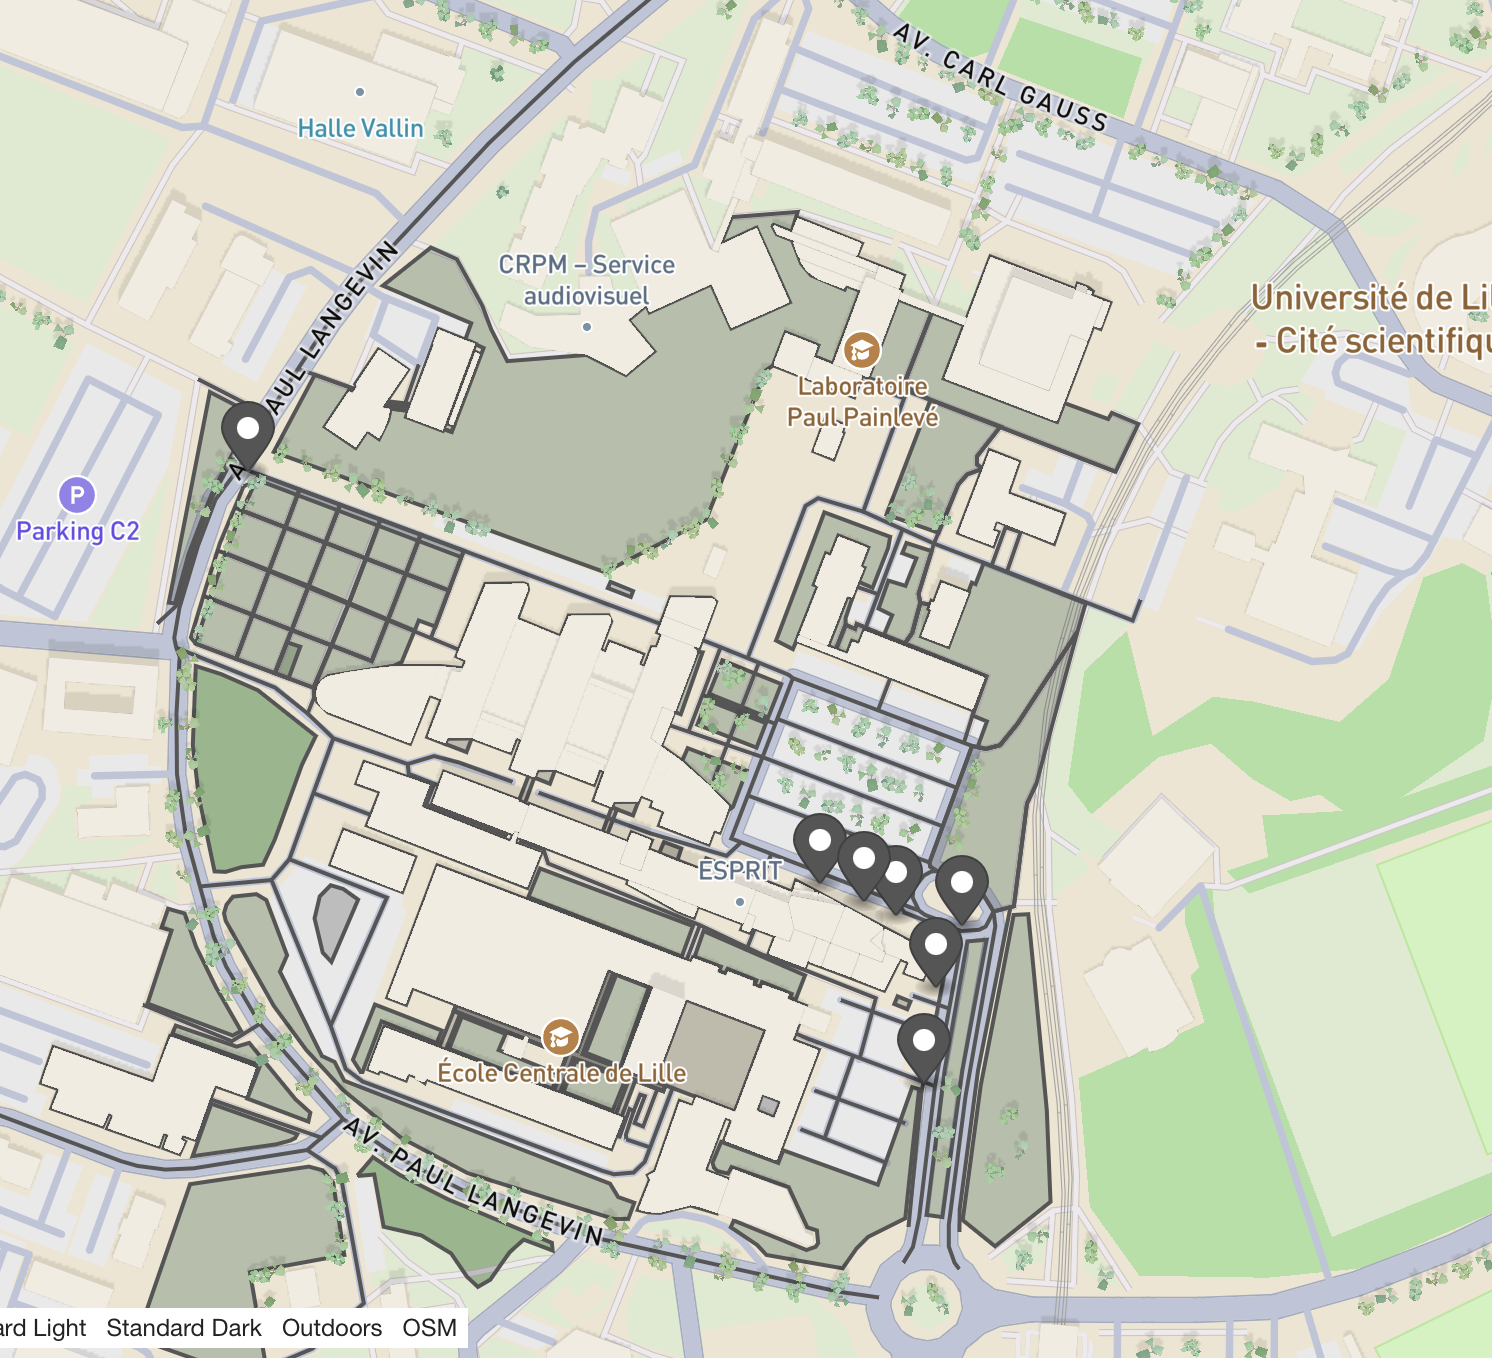
\includegraphics[height=3.5cm]{zone.png}};
        \node[inner sep=0pt, anchor=west] (d) at ([xshift=0.8cm]z.east) {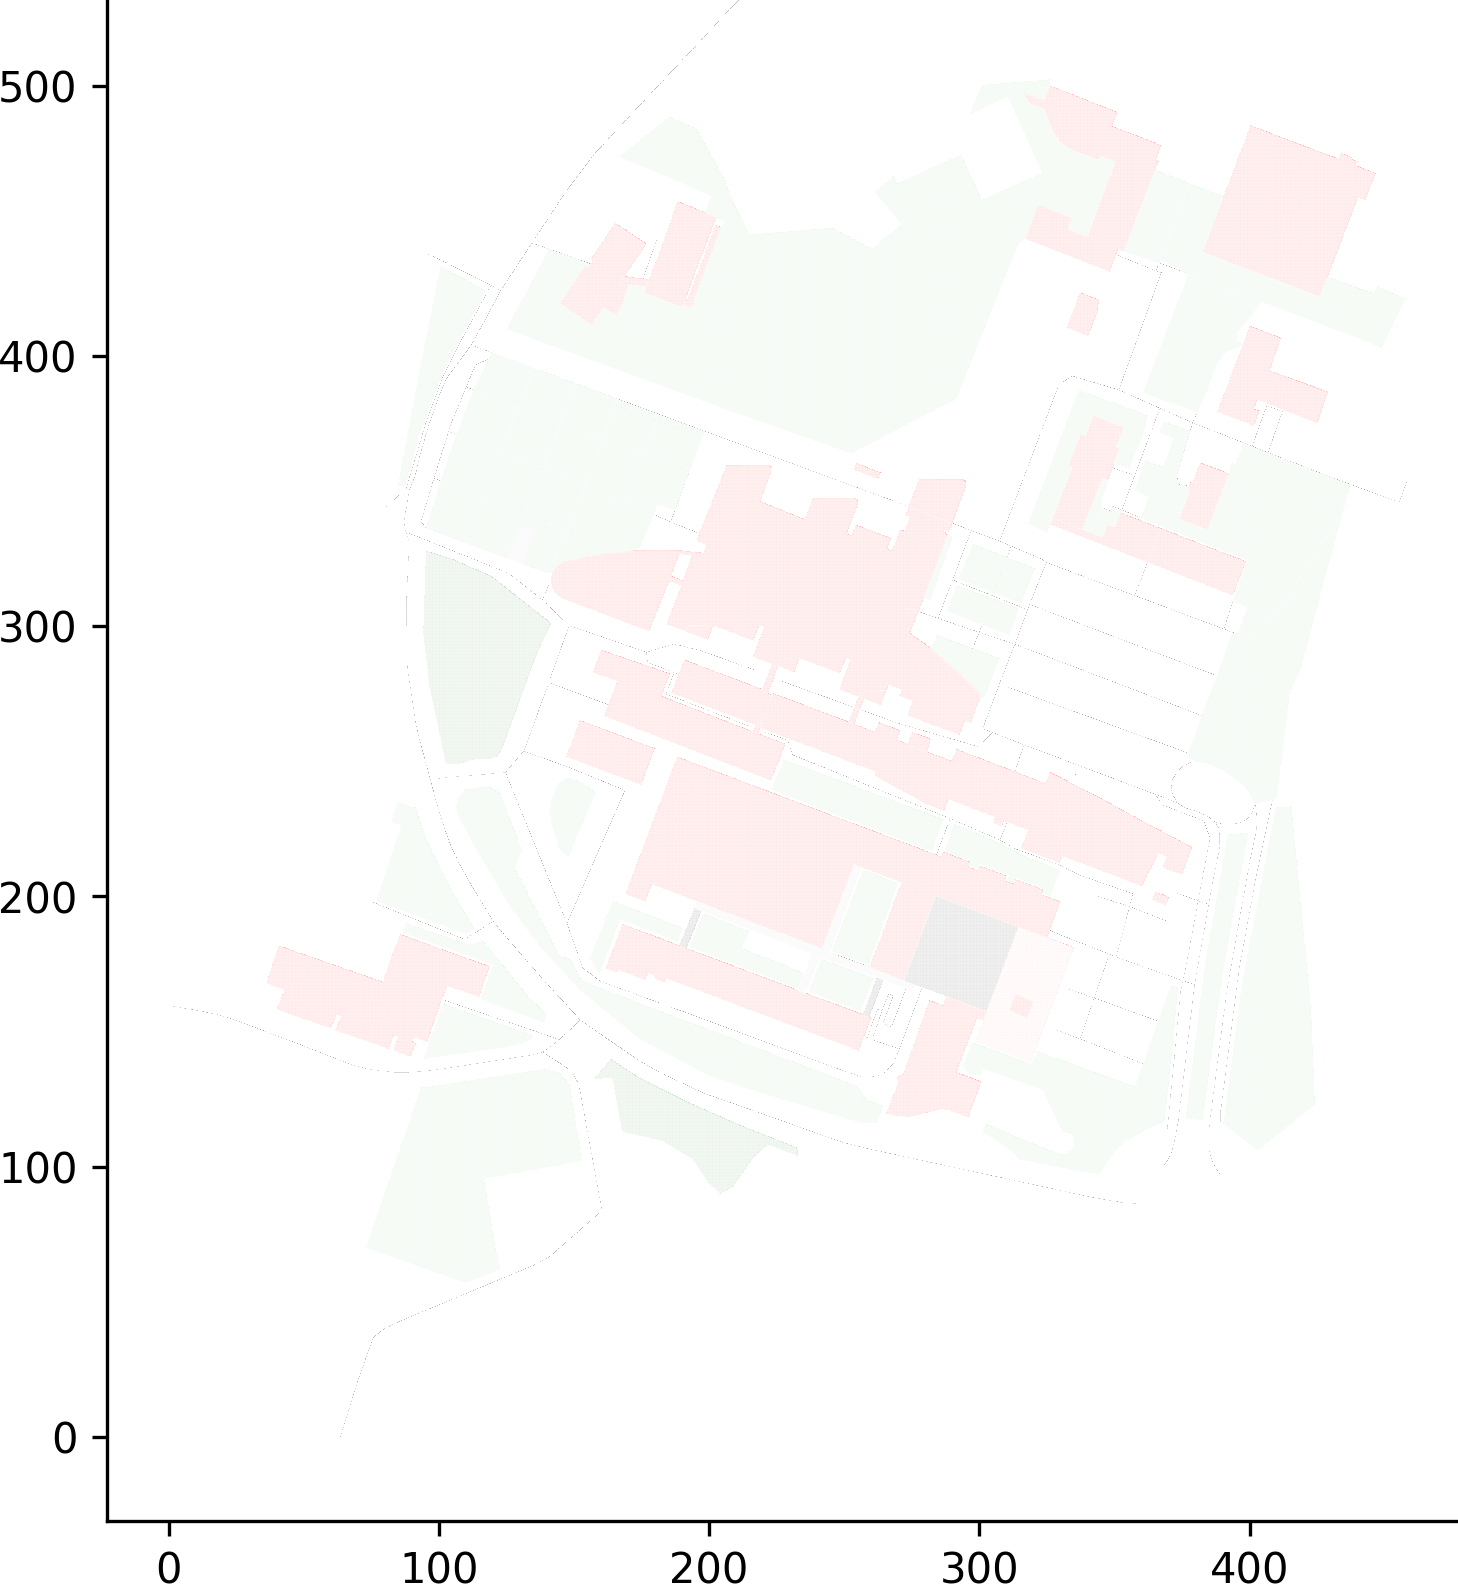
\includegraphics[height=3.5cm]{discretized-map.png}};
        \draw[fleche, very thick] ([xshift=0.1cm]z.east) -- ([xshift=-0.1cm]d.west);
        \node[anchor=north, font=\scriptsize, text=textgray] at (z.south) {Overpass Turbo};
        \node[anchor=north, font=\scriptsize, text=textgray, align=center] at (d.south) {grille discrétisée};
      \end{tikzpicture}
    \end{column}
    \begin{column}{0.42\textwidth}
      \begin{itemize}
        \item Rôles : \alert{référence} de navigation, \alert{vérité terrain}
        \item OSM $\rightarrow$ GeoJSON $\rightarrow$ \alert{grille}\\
              {\footnotesize\color{textgray} GeoPandas, jointure spatiale}
        \item Case à cheval $\rightarrow$ \alert{priorité}\\
              {\footnotesize\color{textgray} bâtiment $>$ route \dots}
        \item Recalage : repère local\\
              + \alert{position / cap initiaux}
      \end{itemize}
    \end{column}
  \end{columns}
\end{frame}

% ----------------------------------------------------------------------
% À DIRE (~50 s)
%  - Jusqu'ici : un seul nœud qui faisait tout, pour un seul robot.
%    Objectif ANR-SOS : une carte sémantique unique, partagée, construite
%    à partir de plusieurs robots.
%  - Séparation en deux nœuds :
%      * PerceptionNode, un par robot : toute la chaîne de fusion
%        (synchro, projection avec la calibration du robot, YOLO,
%        interpolation, loop closure), mais il ne construit plus de
%        carte : il publie ses points déjà dans le repère monde sur
%        /<robot>/semantic_points ;
%      * MapFusionNode, une seule instance : s'abonne aux topics des
%        robots déclarés (paramètre robots), accumule les points de tous
%        les robots et génère la carte commune PÉRIODIQUEMENT (timer ROS 2,
%        paramètre write_interval_sec), plus seulement à l'arrêt.
%  - Message PointCloud2 : position, identifiant numérique du label (ce
%    format n'accepte que des champs numériques, pas de chaînes), une
%    confiance liée à la portée et l'horodatage. La table identifiant ->
%    nom de classe est publiée une seule fois.
%  - Nommage : chaque robot a son namespace (/scout/..., /ranger/...).
%    Pour TF, deux options : un arbre TF séparé par robot (simple, mais
%    plus aucun lien possible entre robots) ou préfixer les repères
%    (scout/base_link) dans un arbre unique -> choix retenu, car il
%    permettra plus tard de relier les repères des robots entre eux.
% ----------------------------------------------------------------------
\begin{frame}{Extension multi-robots}
  \centering
  \begin{tikzpicture}[font=\scriptsize]
    \node[capteur=2.2cm, minimum height=0.95cm] (s) at (0,1.05) {\textbf{Scout}\\ LiDAR, caméra, LIO};
    \node[capteur=2.2cm, minimum height=0.95cm] (r) at (0,-1.05) {\textbf{Ranger}\\ LiDAR, caméra, LIO};
    \node[boite=2.5cm, minimum height=0.95cm] (ps) at (3.35,1.05) {\texttt{PerceptionNode}\\ {\tiny un par robot}};
    \node[boite=2.5cm, minimum height=0.95cm] (pr) at (3.35,-1.05) {\texttt{PerceptionNode}\\ {\tiny un par robot}};
    \node[donnee=2.6cm, minimum height=1.3cm] (mf) at (8.3,0) {\texttt{MapFusionNode}\\ unique : agrégation\\ {\tiny carte générée périodiquement}};
    \node[sortie=2.0cm, minimum height=0.95cm] (out) at (11.4,0) {Carte commune\\ {\tiny\mdseries GeoJSON}};
    \draw[fleche] (s) -- (ps);
    \draw[fleche] (r) -- (pr);
    \draw[fleche] (ps.east) -| node[pos=0.3, above, font=\tiny\ttfamily] {/scout/semantic\_points} (mf.north);
    \draw[fleche] (pr.east) -| node[pos=0.3, below, font=\tiny\ttfamily] {/ranger/semantic\_points} (mf.south);
    \draw[fleche] (mf) -- (out);
  \end{tikzpicture}\par
  \vspace{0.35cm}
  \begin{columns}[T]
    \begin{column}{0.47\textwidth}
      \begin{itemize}
        \item \texttt{PointCloud2} : $x, y, z$, \alert{id du label},\\ confiance, horodatage
        \item Table id $\leftrightarrow$ classe publiée \alert{une fois}
      \end{itemize}
    \end{column}
    \begin{column}{0.47\textwidth}
      \begin{itemize}
        \item \alert{Namespaces} : \texttt{/scout/\dots}, \texttt{/ranger/\dots}
        \item TF : repères \alert{préfixés} (\texttt{scout/base\_link})\\ dans un \alert{arbre unique}
      \end{itemize}
    \end{column}
  \end{columns}
\end{frame}

% ======================================================================
%  PARTIE 6 -- Expérimentations et résultats                 (~4 min)
% ======================================================================
\section{Expérimentations et résultats}

% ----------------------------------------------------------------------
% À DIRE (~30 s)
%  - Deux robots terrestres AgileX :
%      * Scout Mini : compact, 4 roues motrices indépendantes, 10 kg de
%        charge utile, 1,5 m/s max, ~3 h d'autonomie, pentes jusqu'à 30° ;
%      * Ranger : 4 roues indépendantes, omnidirectionnel, jusqu'à 150 kg,
%        2,6 m/s max, ~4 h d'autonomie, batteries remplaçables à chaud.
%  - Tous deux équipés du kit R&D de Génération Robots : LiDAR, caméra de
%    profondeur Intel RealSense D435, GPS RTK, IMU, calculateur embarqué
%    avec les pilotes ROS 2.
%  - Acquisitions enregistrées (bags) puis rejouées, dans la même zone
%    (près du bâtiment ESPRIT) -> carte a priori disponible pour les deux :
%      * Ranger : bag d'une acquisition multi-robots existante (drone +
%        Ranger), 8 min, que je n'ai pas réalisée moi-même ;
%      * Scout : acquisition que j'ai pilotée (avec Gérald Dherbomez,
%        plateforme PRETIL) : bag court, facile à rejouer, et surtout une
%        vraie boucle fermée pour tester la loop closure.
% ----------------------------------------------------------------------
\begin{frame}{Plateformes et acquisitions}
  \begin{columns}[c]
    \begin{column}{0.3\textwidth}
      \centering
      \adjincludegraphics[width=\linewidth, trim={{0.08\width} {0.1\height} {0.09\width} {0.22\height}}, clip]{scout.png}\\[2pt]
      \textbf{Scout Mini}\\
      {\footnotesize\color{textgray} 1,5 m/s \textbullet\ 10 kg \textbullet\ 3 h}
    \end{column}
    \begin{column}{0.3\textwidth}
      \centering
      \adjincludegraphics[width=\linewidth, trim={{0.12\width} {0.08\height} {0.15\width} {0.18\height}}, clip]{ranger.png}\\[2pt]
      \textbf{Ranger}\\
      {\footnotesize\color{textgray} 2,6 m/s \textbullet\ 150 kg \textbullet\ 4 h}
    \end{column}
    \begin{column}{0.34\textwidth}
      \begin{tcolorbox}[carte, title=Kit R\&D (Génération Robots)]
        LiDAR 3D \textbullet\ IMU\\
        Caméra RealSense D435\\
        GPS RTK\\
        PC embarqué + \alert{ROS 2}
      \end{tcolorbox}
    \end{column}
  \end{columns}
  \vspace{0.35cm}
  {\small
  \begin{tabular}{@{}l@{\hspace{0.4cm}}l@{}}
    \textbf{Ranger} & bag existant (drone + Ranger), \alert{8 min} \\
    \textbf{Scout Mini} & acquisition pilotée, \alert{boucle fermée} sur le parking \\
  \end{tabular}\\[3pt]
  $\Rightarrow$ même zone (bâtiment \alert{ESPRIT}) : carte a priori disponible pour les deux\par}
\end{frame}

% ----------------------------------------------------------------------
% À DIRE (~40 s)
%  - Résultats sur le bag du Ranger (8 min), affichés sur la carte a
%    priori (qui sert ici uniquement de fond de carte).
%  - L'information sémantique des cases est cohérente avec la réalité : on
%    retrouve les bâtiments et les arbres, visibles aussi sur la carte de
%    LIO (trajectoire en vert).
%  - La carte 3D permet de mieux visualiser bâtiments et arbres.
%  - Limite : un écart de position avec la carte a priori, dû au manque de
%    précision de la position initiale donnée par le GPS (~5 m d'erreur) ;
%    le magnétomètre s'est révélé inutilisable, l'orientation initiale a
%    donc été recalée visuellement.
% ----------------------------------------------------------------------
\begin{frame}{Résultats : Ranger}
  \centering
  \begin{tabular}{@{}c@{\hspace{0.3cm}}c@{\hspace{0.3cm}}c@{}}
    \adjincludegraphics[height=3.6cm, trim={{0.22\width} {0.38\height} {0.2\width} {0.1\height}}, clip]{ranger_carte_zoom.png} &
    \adjincludegraphics[height=3.6cm, trim={{0.235\width} {0.13\height} {0.18\width} {0.35\height}}, clip]{ranger_liosam.png} &
    \adjincludegraphics[height=3.6cm, trim={{0.0\width} {0.08\height} {0.0\width} {0.0\height}}, clip]{ranger_carte3d.png} \\
    \legende{\shortstack{Carte 2D (pas de 1 m)\\ sur la carte a priori}} &
    \legende{Carte et trajectoire LIO} &
    \legende{Carte sémantique 3D} \\
  \end{tabular}\par
  \vspace{0.2cm}
  {\small \ok\ sémantique \alert{cohérente} (bâtiments, arbres)
   \qquad \ko\ \alert{décalage} : GPS initial ($\sim$5 m)\par}
\end{frame}

% ----------------------------------------------------------------------
% À DIRE (~50 s)
%  - Bag du Scout : un tour complet du parking devant ESPRIT, à vitesse de
%    marche -> vraie loop closure en conditions réelles.
%  - Sans loop closure : la carte est dédoublée, à cause de la dérive de
%    la trajectoire estimée par LIO. À un moment la dérive devient très
%    forte : LIO retrouve ensuite une trajectoire cohérente mais avec une
%    pente très exagérée, alors que le robot est resté à plat.
%    Hypothèse : données IMU brutes, non filtrées (pas de dérive de ce
%    type avec le Ranger).
%  - Avec loop closure : carte nettement plus cohérente avec le chemin
%    réel. L'optimiseur ne corrige pas que la dernière pose : il
%    redistribue la correction sur toute la trajectoire -> c'est
%    exactement ce que fait le recalcul complet des points.
%  - Remarque : avec loop closure, même le DÉBUT de la carte change
%    légèrement d'orientation par rapport au cap initial renseigné à la
%    main, car la pose de départ n'est pas figée dans l'optimisation.
%  - (Slide de secours en annexe : bag lu à partir de 60 s.)
% ----------------------------------------------------------------------
\begin{frame}{Résultats : Scout Mini et loop closure}
  \centering
  % images centrées verticalement (\raisebox) pour aligner les étiquettes de ligne
  \begin{tabular}{@{}c@{\hspace{0.25cm}}c@{\hspace{0.5cm}}c@{}}
    & \textbf{Sans loop closure} & \textbf{Avec loop closure} \\[3pt]
    \rotatebox[origin=c]{90}{\scriptsize\color{textgray} carte sémantique} &
    \raisebox{-0.5\height}{\adjincludegraphics[height=2.45cm, trim={{0.521\width} {0.300\height} {0.122\width} {0.455\height}}, clip]{scout_sansloop.png}} &
    \raisebox{-0.5\height}{\adjincludegraphics[height=2.45cm, trim={{0.503\width} {0.304\height} {0.140\width} {0.440\height}}, clip]{scoot_loop.png}} \\[1.3cm]
    \rotatebox[origin=c]{90}{\scriptsize\color{textgray} trajectoire LIO} &
    \raisebox{-0.5\height}{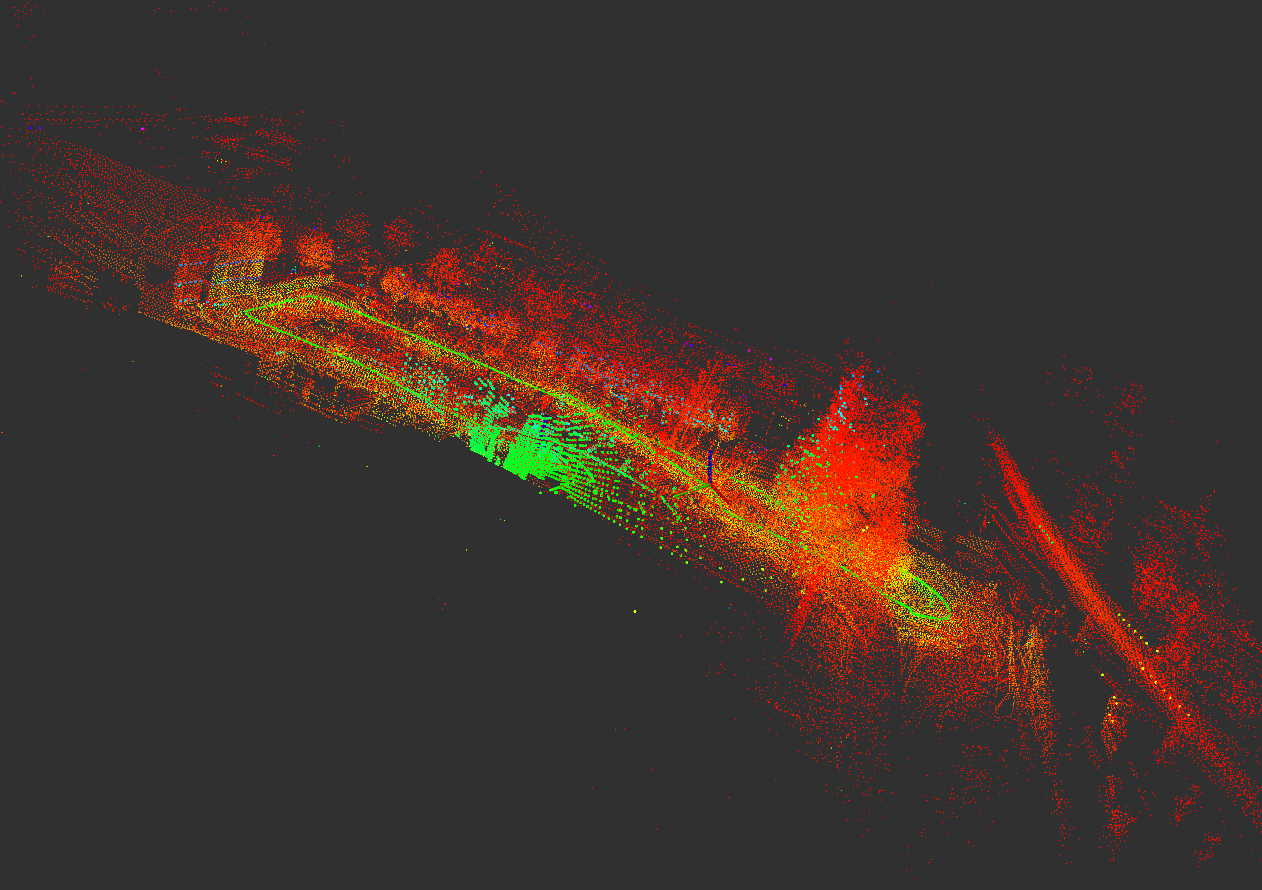
\includegraphics[height=2.45cm]{scoot_liosam_sansloop.png}} &
    \raisebox{-0.5\height}{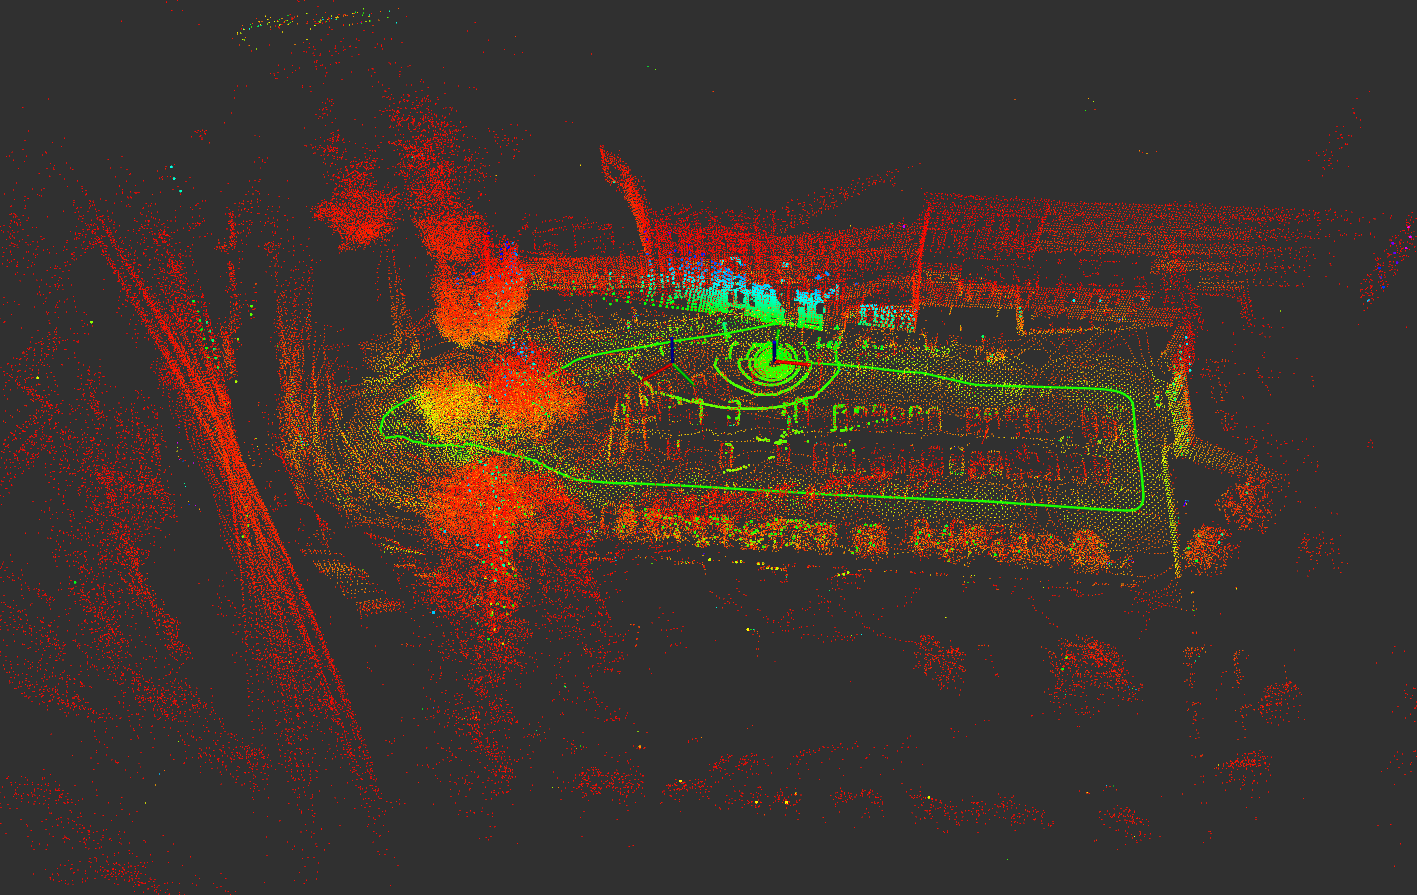
\includegraphics[height=2.45cm]{scoot_liosam_loop.png}} \\[1.35cm]
    & {\footnotesize \ko\ \alert{dérive} : carte dédoublée, pente exagérée}
    & {\footnotesize \ok\ carte \alert{cohérente}, correction globale} \\
  \end{tabular}
\end{frame}

% ----------------------------------------------------------------------
% À DIRE (~40 s)
%  - Test multi-robots avec les deux bags (Ranger et Scout) rejoués en
%    même temps : ce n'est donc pas du multi-robots temps réel (les
%    acquisitions n'ont pas été faites simultanément).
%  - Mais cela valide les bases : les deux cartes sont agrégées dans une
%    carte commune, un seul fichier GeoJSON, sans conflit de topics ni de
%    repères TF.
%  - Limite : si une même case est vue par les deux robots, les deux
%    informations sont gardées -> deux lignes pour la même case dans le
%    GeoJSON -> il faudra une fusion (bayésienne).
%  - La loop closure fonctionne aussi en multi-robots, mais avec les deux
%    bags + deux frameworks sur la même machine, les pertes de données
%    sont encore plus importantes.
% ----------------------------------------------------------------------
\begin{frame}{Résultats : multi-robots}
  \begin{columns}[c]
    \begin{column}{0.53\textwidth}
      \centering
      \begin{tikzpicture}
        % carte complète (hauteur 5 cm -> largeur 3,855 cm) et zoom sur les deux zones
        \node[inner sep=0pt, anchor=south west] (full) at (0,0) {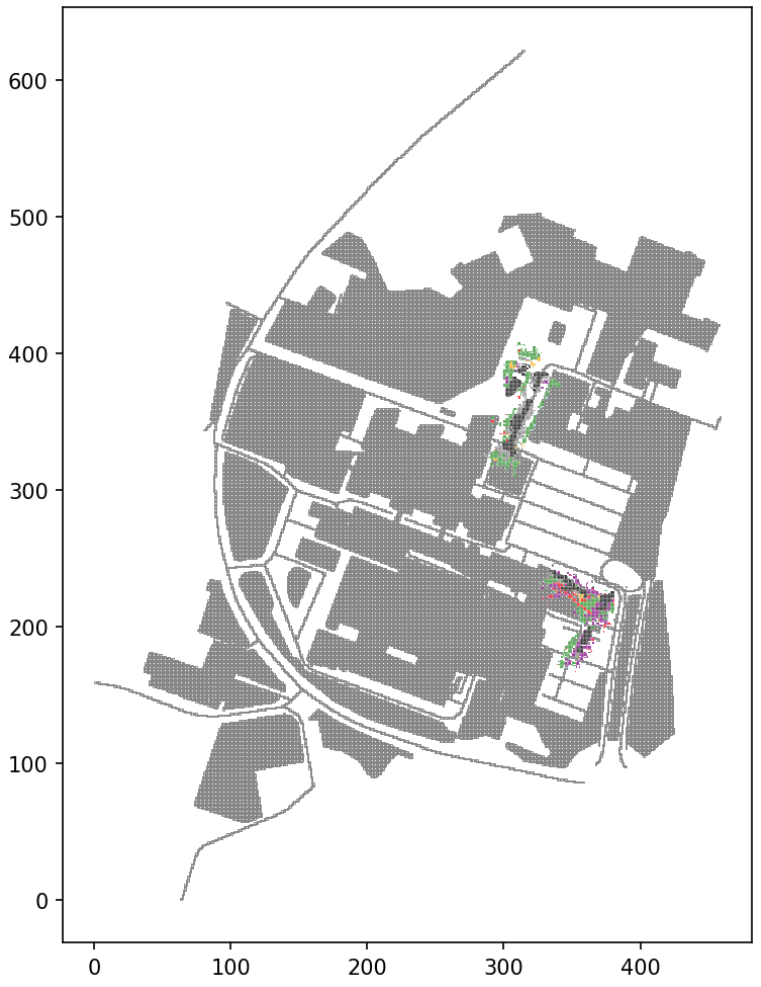
\includegraphics[height=5cm]{multi.png}};
        \node[inner sep=0pt, anchor=south west] (zoom) at (4.15,0)
          {\adjincludegraphics[height=5cm, trim={{0.565\width} {0.291\height} {0.106\width} {0.304\height}}, clip]{multi.png}};
        \draw[accent, thick] (2.178,1.455) rectangle (3.446,3.48);
        \draw[accent, thin] (3.446,3.48) -- (zoom.north west);
        \draw[accent, thin] (3.446,1.455) -- (zoom.south west);
        \draw[accent, thick] (zoom.south west) rectangle (zoom.north east);
        \node[anchor=north, font=\scriptsize, text=textgray] at (full.south) {carte commune};
        \node[anchor=north, font=\scriptsize, text=textgray] at (zoom.south) {zoom};
        \node[anchor=east, fill=white, inner sep=1pt, font=\tiny\bfseries, text=primaryblue] at ([xshift=-2pt, yshift=-1.4cm]zoom.north east) {Ranger};
        \node[anchor=east, fill=white, inner sep=1pt, font=\tiny\bfseries, text=primaryblue] at ([xshift=-2pt, yshift=1.1cm]zoom.south east) {Scout};
      \end{tikzpicture}
    \end{column}
    \begin{column}{0.45\textwidth}
      \begin{itemize}
        \item 2 bags rejoués \alert{ensemble}\\ {\footnotesize\color{textgray} (pas de temps réel)}
        \item[\ok] \alert{un seul GeoJSON} commun
        \item[\ok] pas de conflit de topics ni de TF
        \item[\ko] case vue 2 fois $\rightarrow$ 2 entrées\\ $\Rightarrow$ \alert{fusion bayésienne} à faire
        \item[\ko] loop closure + 2 robots sur 1 PC\\ $\rightarrow$ pertes de données
      \end{itemize}
    \end{column}
  \end{columns}
\end{frame}

% ======================================================================
%  PARTIE 7 -- Conclusion et perspectives                    (~1 min 30)
% ======================================================================
\section{Conclusion et perspectives}

% ----------------------------------------------------------------------
% À DIRE (~40 s)
%  - Objectif du stage : une brique de cartographie sémantique coopérative
%    pour des flottes de robots en extérieur (ANR-SOS).
%  - Réalisé : un framework ROS 2 qui projette les nuages LiDAR sur les
%    images, les étiquette avec YOLO, les place dans le repère monde grâce
%    à l'odométrie LiDAR-inertielle de LIO, et génère une carte sémantique
%    2D / 3D en GeoJSON ; avec prise en compte des loop closures, d'une
%    carte a priori, et une architecture multi-robots.
%  - Validé sur KITTI puis sur deux robots AgileX réels (Scout Mini et
%    Ranger).
%  - C'est une première base fonctionnelle, pensée pour accueillir les
%    futures contributions du laboratoire (contraintes GPS multi-robots,
%    planification, navigation).
% ----------------------------------------------------------------------
\begin{frame}{Bilan}
  \begin{columns}[c]
    \begin{column}{0.62\textwidth}
      \begin{itemize}
        \item[\ok] Framework \alert{ROS 2} : \alert{LIO + YOLO}\\
              $\rightarrow$ carte sémantique \alert{2D / 3D} (GeoJSON)
        \item[\ok] Prise en compte des \alert{loop closures}
        \item[\ok] \alert{Carte a priori} OpenStreetMap
        \item[\ok] Architecture \alert{multi-robots}
        \item[\ok] Validé sur \alert{KITTI}, \alert{Scout Mini} et \alert{Ranger}
      \end{itemize}
    \end{column}
    \begin{column}{0.34\textwidth}
      \centering
      \adjincludegraphics[height=4.2cm, trim={{0.22\width} {0.38\height} {0.2\width} {0.1\height}}, clip]{ranger_carte_zoom.png}\\
      \legende{Carte sémantique du Ranger}
    \end{column}
  \end{columns}
  \vspace{0.35cm}
  \begin{tcolorbox}[question, width=0.85\textwidth]
    Une \alert{première base fonctionnelle}, validée en conditions réelles,\\
    pour la cartographie sémantique coopérative du projet ANR-SOS
  \end{tcolorbox}
\end{frame}

% ----------------------------------------------------------------------
% À DIRE (~40 s)
%  - Intégrer la sémantique DANS LIO : aujourd'hui LIO et YOLO sont deux
%    modules indépendants (avantage : on peut faire évoluer l'un sans
%    toucher l'autre). Mais les labels, gérés hors de LIO, doivent être
%    resynchronisés à chaque loop closure. Si LIO est confirmé, ajouter le
%    label comme propriété de chaque point dans LIO : les corrections de
%    trajectoire s'appliqueraient automatiquement, sans recalcul externe.
%  - Position / orientation initiales : moyenner plusieurs mesures GPS au
%    lieu d'une seule ; pour le cap, un petit script qui fait avancer le
%    robot de quelques mètres et en déduit l'orientation par GPS (le
%    magnétomètre étant inutilisable).
%  - Fusion bayésienne : remplacer le "label dominant" par une fusion qui
%    tient compte de la fiabilité de chaque source (plusieurs robots,
%    carte a priori). Pas eu le temps de la mettre en œuvre.
%  - Tests réels : faire tourner le framework en temps réel sur le
%    calculateur embarqué de chaque robot, puis en multi-robots. Et pour
%    un autre environnement (forêt), ré-entraîner YOLO : le modèle actuel
%    est entraîné sur Cityscapes (scènes urbaines).
% ----------------------------------------------------------------------
\begin{frame}{Perspectives}
  \vfill
  \begin{tcbraster}[raster columns=2, raster equal height, raster column skip=0.4cm, raster row skip=0.3cm]
    \begin{tcolorbox}[carte, title=Sémantique intégrée à LIO]
      label porté par chaque point dans LIO\\
      $\rightarrow$ loop closures \alert{sans recalcul externe}
    \end{tcolorbox}
    \begin{tcolorbox}[carte, title=Initialisation des robots]
      moyenne GPS, court déplacement\\
      $\rightarrow$ \alert{position et cap} initiaux fiables
    \end{tcolorbox}
    \begin{tcolorbox}[carte, title=Fusion bayésienne]
      robots + carte a priori\\
      $\rightarrow$ selon la \alert{fiabilité} de chaque source
    \end{tcolorbox}
    \begin{tcolorbox}[carte, title=Tests en conditions réelles]
      \alert{temps réel} embarqué, puis multi-robots\\
      YOLO ré-entraîné hors milieu urbain
    \end{tcolorbox}
  \end{tcbraster}
  \vfill
\end{frame}

% ----------------------------------------------------------------------
% À DIRE (~10 s)
%  - Remercier le jury, puis ouvrir aux questions.
%  - Slides de secours en annexe (après celle-ci) : paramètres de loop
%    closure, calcul du champ ring, format GeoJSON, Scout avec bag
%    décalé de 60 s.
% ----------------------------------------------------------------------
\begin{frame}[plain]
  \centering
  \vfill
  {\Huge\bfseries\color{primaryblue} Merci pour votre attention\par}
  \vspace{0.35cm}
  {\color{accent}\rule{3cm}{2pt}\par}
  \vspace{0.35cm}
  {\LARGE\color{accent} Questions ?\par}
  \vfill
  
\includegraphics[height=0.9cm]{logo_labo.png}\hspace{1cm}%
  \adjincludegraphics[height=0.9cm, trim={{0.04\width} {0.31\height} {0.04\width} {0.31\height}}, clip]{logo_etablissement.png}
  \vspace{0.3cm}
\end{frame}


% Slides de secours (après "Questions ?") : non comptées dans la numérotation
\appendix
% ======================================================================
%  ANNEXES -- slides de secours, à montrer seulement si une question
%  porte dessus (non comptées dans la numérotation principale)
% ======================================================================

% ----------------------------------------------------------------------
% SI QUESTION sur le réglage de la loop closure
%  - Le réglage de ces paramètres, surtout le rayon de recherche et le
%    seuil de fitness, fixe la sensibilité de la détection : rayon trop
%    grand ou seuil trop permissif -> fausses détections ; valeurs trop
%    strictes -> vraies boucles manquées.
%  - Sur KITTI (bag sans vraie boucle), j'ai forcé une loop closure en
%    réduisant fortement le délai minimal (historyKeyframeSearchTimeDiff),
%    uniquement pour tester la communication framework <-> LIO.
% ----------------------------------------------------------------------
\begin{frame}{Annexe : paramètres de loop closure de LIO}
  \centering
  \small
  \begin{tabular}{@{}l c l@{}}
    \toprule
    \textbf{Paramètre} & \textbf{Défaut} & \textbf{Rôle} \\
    \midrule
    \texttt{loopClosureEnableFlag}         & --     & active / désactive la détection \\
    \texttt{loopClosureFrequency}          & 1 Hz   & fréquence des tentatives \\
    \texttt{historyKeyframeSearchRadius}   & 15 m   & rayon de recherche des candidates \\
    \texttt{historyKeyframeSearchTimeDiff} & 30 s   & écart temporel minimal \\
    \texttt{historyKeyframeSearchNum}      & 25     & keyframes par sous-carte (ICP) \\
    \texttt{historyKeyframeFitnessScore}   & 0,3    & seuil ICP (plus bas = plus strict) \\
    \bottomrule
  \end{tabular}\par
  \vspace{0.4cm}
  {\small rayon trop grand / seuil permissif $\rightarrow$ \alert{fausses boucles}\\[2pt]
   valeurs trop strictes $\rightarrow$ \alert{boucles manquées}\par}
\end{frame}

% ----------------------------------------------------------------------
% SI QUESTION sur le champ ring (KITTI)
%  - Chaque nappe du LiDAR correspond à un angle d'élévation fixe ; on
%    rattache le point à la nappe dont l'angle est le plus proche.
%  - D = distance du point au LiDAR, theta = arcsin(z / D), puis on ramène
%    theta dans [0, N] entre theta_min = -24,8° et theta_max = 2°
%    (Velodyne de KITTI, N = 64).
%  - Hypothèse : espacement angulaire uniforme entre nappes -> c'est une
%    approximation.
% ----------------------------------------------------------------------
\begin{frame}{Annexe : calcul du champ \texttt{ring} (KITTI)}
  \begin{columns}[c]
    \begin{column}{0.52\textwidth}
      \centering
      \begin{tikzpicture}[scale=1.05, >={Stealth}]
        \coordinate (O) at (0,0);
        \foreach \ang in {-15,-9,-3,3,9,15,21} {
          \draw[gray!55, thin] (O) -- (\ang:4.6);
        }
        \node[gray!70] at (-15:5.05) {\scriptsize ring $0$};
        \node[gray!70] at (21:5.15) {\scriptsize ring $N{-}1$};
        \draw[dashed] (O) -- (4.8,0);
        \node[below right] at (4.8,0) {\scriptsize $\theta = 0$};
        \coordinate (P) at (6:4);
        \draw[thick, ->, accent] (O) -- (P);
        \fill[accent] (P) circle (1.8pt);
        \node[above right=1pt] at (P) {$P(x,y,z)$};
        \node[above=1pt] at (6:1.9) {\scriptsize $D$};
        \draw (0.9,0) arc (0:6:0.9);
        \node at (1.45,0.11) {\scriptsize $\theta$};
        \fill (O) circle (2pt);
        \node[left=2pt] at (O) {\scriptsize LiDAR};
      \end{tikzpicture}
    \end{column}
    \begin{column}{0.44\textwidth}
      \[
        D = \sqrt{x^2 + y^2 + z^2}
      \]
      \[
        \theta = \arcsin\!\left(\frac{z}{D}\right)
      \]
      \[
        \text{ring} = \frac{\theta - \theta_{\min}}{\theta_{\max} - \theta_{\min}} \times N
      \]
      \vspace{0.1cm}
      \begin{itemize}
        \item Velodyne KITTI : $N = 64$,\\ $\theta_{\min} = -24{,}8^\circ$, $\theta_{\max} = 2^\circ$
        \item \alert{Approximation} : nappes régulièrement espacées
      \end{itemize}
    \end{column}
  \end{columns}
\end{frame}

% ----------------------------------------------------------------------
% SI QUESTION sur le format de sortie (carte a priori)
%  - Une "feature" GeoJSON par case : centre de la case, label, identifiant
%    OSM d'origine ; le polygone de la case reste disponible.
%  - Système de coordonnées : Lambert-93 (EPSG:2154), ramené dans un
%    repère local en soustrayant l'origine de la carte.
% ----------------------------------------------------------------------
\begin{frame}[fragile]{Annexe : format GeoJSON (\texttt{export\_grid.geojson})}
  \begin{columns}[c]
    \begin{column}{0.66\textwidth}
\begin{semiverbatim}\scriptsize
\{
  "type": "FeatureCollection",
  "name": "export_grid",
  "crs": \{ "type": "name", "properties":
    \{ "name": "urn:ogc:def:crs:EPSG::2154" \} \},
  "features": [
    \{ "type": "Feature",
      "properties": \{
        "center_x": 0.5, "center_y": 159.5,
        "label": "road", "id": "way/154556229" \},
      "geometry": \{ "type": "Polygon",
        "coordinates": [ [ [ 0.0, 159.0 ], [ 1.0, 159.0 ],
          [ 1.0, 160.0 ], [ 0.0, 160.0 ],
          [ 0.0, 159.0 ] ] ] \} \},
    ...
  ]
\}
\end{semiverbatim}
    \end{column}
    \begin{column}{0.3\textwidth}
      \begin{itemize}
        \item 1 case = 1 \alert{feature}
        \item centre, \alert{label}, id OSM
        \item polygone de la case
        \item Lambert-93 ({\NoAutoSpacing\alert{EPSG:2154}})
      \end{itemize}
    \end{column}
  \end{columns}
\end{frame}

% ----------------------------------------------------------------------
% SI QUESTION sur la forte dérive du Scout
%  - Essai complémentaire : lecture du bag du Scout à partir de 60 s, pour
%    éviter la phase de forte dérive observée au début de l'acquisition.
%  - (À adapter : ces figures ne sont pas commentées dans le rapport, dire
%    ce que tu en as conclu.)
% ----------------------------------------------------------------------
\begin{frame}{Annexe : Scout, bag lu à partir de 60 s}
  \centering
  \begin{tabular}{@{}c@{\hspace{0.5cm}}c@{}}
    \adjincludegraphics[height=4.6cm, trim={{0.485\width} {0.26\height} {0.138\width} {0.479\height}}, clip]{scoot_loop_differe.png} &
    \adjincludegraphics[height=4.6cm, trim={{0.25\width} {0.2\height} {0.1\width} {0.12\height}}, clip]{scoot_liosam_differe_loop.png} \\
    \legende{Carte sémantique, loop closure activée} &
    \legende{Trajectoire LIO} \\
  \end{tabular}
\end{frame}


\end{document}
